\documentclass{ieeeojies}
\usepackage{cite}
\usepackage{amsmath,amssymb,amsfonts}
\usepackage{algorithmic}
\usepackage{graphicx}
\usepackage{textcomp}
\usepackage{booktabs}
\usepackage{tabularx}
\usepackage[caption=false,font=footnotesize]{subfig}
\usepackage{url}
\usepackage[hidelinks]{hyperref}

\def\BibTeX{{\rm B\kern-.05em{\sc i\kern-.025em b}\kern-.08em
    T\kern-.1667em\lower.7ex\hbox{E}\kern-.125emX}}

\newcommand{\etal}{\textit{et~al.}}
\renewcommand{\topfraction}{0.95}
\renewcommand{\bottomfraction}{0.85}
\renewcommand{\textfraction}{0.05}
\renewcommand{\floatpagefraction}{0.85}
\renewcommand{\dbltopfraction}{0.95}
\renewcommand{\dblfloatpagefraction}{0.85}

\begin{document}

\title{Automatic Generation of Simulation-Based Digital Twins From Asset Administration Shells}

\author{\uppercase{Tiago Gouveia}\authorrefmark{1},
\uppercase{Nelson Freitas}\authorrefmark{1,2}, and
\uppercase{Andr{\'e} Dion{\'i}sio Rocha}\authorrefmark{1,2}, \IEEEmembership{Member, IEEE}}
\address[1]{Department of Electrical and Computer Engineering, NOVA School of Science and Technology (NOVA FCT), NOVA University of Lisbon, 2829-516 Caparica, Portugal (e-mail: td.gouveia@campus.fct.unl.pt; n.freitas@campus.fct.unl.pt; ad.rocha@fct.unl.pt)}
\address[2]{Centre of Technology and Systems (CTS), UNINOVA, 2829-516 Caparica, Portugal}
\tfootnote{This work was funded in part by the Portuguese Foundation for Science and Technology (FCT) under the Center of Technology and Systems (CTS) program UID/00066/2025. DOI: \url{https://doi.org/10.54499/UID/00066/2025}}

\markboth
{Gouveia \headeretal: Automatic Generation of Simulation-Based Digital Twins From Asset Administration Shells}
{Gouveia \headeretal: Automatic Generation of Simulation-Based Digital Twins From Asset Administration Shells}

\corresp{Corresponding author: Tiago Gouveia (e-mail: td.gouveia@campus.fct.unl.pt).}

\begin{abstract}
Reconfigurable manufacturing systems require digital twins that can follow the shop floor as machines are added, moved, or replaced. In practice, however, simulation-based digital twins are still assembled by hand inside proprietary tools from manufacturing models that lack kinematic pivots and sensor volumes, and every change in layout or wiring forces the virtual scene and its controller address mappings to be rebuilt. This paper presents an open, model-driven framework that generates and synchronizes simulation-based digital twins directly from standardized Asset Administration Shells. Each asset is described once in a self-contained package that combines its 3D geometry, kinematic behavior, virtual input/output pins, rule-triggered control sequences, and network endpoint through five dedicated submodels. The framework is organized into three decoupled layers, preceded by an optional geometric digitization stage: no-code semantic authoring, storage and discovery through Eclipse BaSyx microservices, and a Unity runtime that assembles the scene procedurally in memory and executes it either for virtual commissioning or as a live digital twin synchronized with an industrial programmable logic controller, using sensor-triggered snapping to cancel physics drift. The framework was validated on a modular flexible manufacturing system conveyor bench and through 800 stress-test runs scaling from 5 to 1000 conveyor modules. The pilot bench is instantiated from a cold start in 2.79 s and runs at about 490 frames per second, while the stress tests show stable real-time execution up to 250 modules and mean frame rates above 60 frames per second up to 500 modules.
\end{abstract}

\begin{keywords}
Asset Administration Shell (AAS), Cyber-Physical Production Systems (CPPS), Digital Twin, Industry~4.0, Procedural Generation, Reconfigurable Manufacturing Systems, Virtual Commissioning.
\end{keywords}

\titlepgskip=-15pt

\maketitle

%=============================================================================
\section{Introduction}
\label{sec:introduction}
%=============================================================================

Modern manufacturing enterprises face growing pressure to adapt production lines to fluctuating market demand, shorter product lifecycles, and high-mix, low-volume customization \cite{Khan2025,Rocha2024}. Traditional Dedicated Manufacturing Systems (DMS) were engineered around rigid topologies and hardwired machinery to produce large volumes of identical goods. Smart manufacturing instead relies on Reconfigurable Manufacturing Systems (RMS) and Cyber-Physical Production Systems (CPPS), in which conveyors, processing stations, and robotic cells can be added, swapped, or rearranged with minimal downtime \cite{Abdel-Aty2022,AshtariTalkhestani2019}.

In this context, the Digital Twin (DT) has become a key enabler of Virtual Commissioning (VC), operational monitoring, and closed-loop validation of control logic \cite{Tao2019,Striffler2023}. Whereas static 3D models and Digital Shadows (DS) only offer manual or unidirectional data flows, a DT maintains automated, bidirectional synchronization between a physical asset and its virtual counterpart \cite{Kritzinger2018,Pajpach2023}: sensor telemetry updates the simulation state, and decisions taken in the virtual environment can be dispatched back to the Programmable Logic Controllers (PLCs) on the shop floor. To prevent multi-vendor fragmentation, Plattform Industrie~4.0 proposed the Reference Architectural Model Industrie~4.0 (RAMI~4.0, IEC~63088) \cite{Pajpach2025}, at whose core lies the Asset Administration Shell (AAS, IEC~63278). Maintained by the Industrial Digital Twin Association (IDTA), the AAS is the standardized digital representation of an asset, organizing its mechanical, electrical, operational, and communication data into interoperable submodels \cite{Lu2025}.

Despite these promises, building and maintaining simulation-based DTs remains a major engineering effort, especially for Small and Medium Enterprises (SMEs) \cite{Gil2024}. The first obstacle is geometric. Factory machines are designed with mechanical CAD assemblies intended for manufacturing, which contain dense tessellations, fasteners, and internal parts and must be converted before game engines can use them \cite{Chowdhury2025}. More importantly, CAD exports flatten the assembly and discard the local pivots, motion axes, stroke limits, and trigger volumes that a physics runtime needs in order to move parts and detect workpieces. The second obstacle is the construction of the virtual scene itself. Mainstream simulation suites require engineers to place machines manually inside proprietary editors, script their kinematics by hand, and compile static scenes \cite{Striffler2023}, so every time a conveyor is added or rearranged on the floor the simulation project must be rebuilt, and the model gradually drifts out of date \cite{Alexopoulos2025}. The third obstacle is the separation between simulation and control hardware. Moving from offline VC to an operational DT connected to field PLCs usually means re-mapping signal tags and I/O addresses by hand across several tools, which is slow and error-prone \cite{Luder2020,Gollner2022}. Together, these bottlenecks explain why conventional tools struggle in agile CPPS environments \cite{Rocha2024}.

This work therefore investigates the following research question: \textit{how can standardized Asset Administration Shells be used to procedurally assemble and synchronize interactive, simulation-based Digital Twins at runtime?} To answer it, the paper proposes, implements, and evaluates an open, layered, model-driven DT framework. Its first contribution is the framework itself, a procedural pipeline that replaces pre-compiled simulation projects by instantiating 3D hierarchies, physics colliders, and network bindings directly from AASX packages at runtime. The second contribution is a unified AAS submodel schema that links 3D geometry (\textit{VisualStructure}), kinematic behavior and trigger volumes (\textit{BehaviorMapping}), electrical I/O terminals (\textit{VirtualPins}), rule-triggered control sequences (\textit{ControlLogic}), and communication bindings (\textit{NetworkEndpoint}) in a single self-describing package. The third contribution is a no-code authoring tool that binds virtual sensors and actuators to the modeled geometry, edits control logic visually, and compiles standard AASX packages with the Eclipse BaSyx Python software development kit (SDK). The fourth contribution is an empirical evaluation on a physical modular Flexible Manufacturing System (FMS) bench controlled by an Industrial Shields PLC running FreeRTOS, complemented by 800 stress-test runs scaling up to 1000 conveyor modules.

%=============================================================================
\section{Related Work}
\label{sec:related_work}
%=============================================================================

\subsection{Cyber-Physical Production Systems}
\label{sec:rw_cpps}

Cyber-Physical Systems (CPS) integrate computation, networking, and physical processes, coupling embedded controllers, sensors, and actuators with the software that monitors and coordinates them \cite{Abdel-Aty2022}. Their application to manufacturing, the CPPS, is the operational backbone of Industry~4.0 \cite{Kagermann2022,Hermann2016}: networked machines expose their state, coordinate their actions, and can be reorganized in software rather than rewired by hand \cite{AshtariTalkhestani2019}. This capability underpins the shift from dedicated lines, through FMS, to modular and convertible RMS \cite{Khan2025}. Within RAMI~4.0, every asset in such a system becomes an \textit{Industry~4.0 Component}, i.e., the physical asset combined with its AAS \cite{Pajpach2025}. For reconfiguration to be fast in practice, however, the software around the machines must discover, configure, and connect new equipment automatically \cite{Rocha2024,Ahvanouee2025}, and this requirement applies equally to the simulation models that represent the line.

\subsection{Digital Twins and Virtual Commissioning}
\label{sec:rw_dt_vc}

The DT concept was introduced by Grieves for product lifecycle management \cite{Grieves2014} and formalized by NASA as an integrated, multi-physics simulation that mirrors the life of its physical counterpart using sensor data and operational history \cite{Shafto2012}. Since then, the term has been used loosely to designate almost any 3D animation or dashboard, which led Kritzinger \etal \cite{Kritzinger2018} to classify virtual representations by their degree of data coupling. A \textit{Digital Model} exchanges data with the physical system manually in both directions, a \textit{Digital Shadow} receives data automatically from the plant but returns nothing, and only a \textit{Digital Twin} closes the loop with automated, bidirectional synchronization. Reference architectures such as the five-dimensional model of Tao \etal \cite{Tao2019} and the agent-based architecture of Ashtari Talkhestani \etal \cite{AshtariTalkhestani2019} describe how these elements should be organized, while surveys emphasize that a DT should accompany the asset from design to decommissioning \cite{Jones2020,Semeraro2021}.

Virtual Commissioning is the lifecycle phase in which simulation models are used to verify PLC programs, kinematic cycles, and collision paths before the physical plant is built \cite{Lee2014,Striffler2023}. It is usually performed in Model-in-the-Loop (MiL), Software-in-the-Loop (SiL), or Hardware-in-the-Loop (HiL) configurations, the latter coupling a real controller to the virtual plant through simulated sensor and actuator signals \cite{Striffler2023}. Commercial VC tools, however, remain detached from the operational phase. Once the line starts producing, the VC model is typically discarded rather than evolved into an operational DT, because keeping it aligned with the plant requires extensive manual re-engineering \cite{Striffler2023}. In this work, VC is understood in its model-in-the-loop sense: the control sequences that will later be dispatched to the physical controllers are first executed against the virtual plant, so that sequencing errors, interlocks, and timeouts can be detected before the equipment is driven.

\subsection{Semantic Modeling and Interoperability Standards}
\label{sec:rw_standards}

Semantic interoperability in heterogeneous manufacturing environments relies on a stack of complementary open standards \cite{Barnard2024,Ahvanouee2025}. AutomationML (AML, IEC~62714) is an Extensible Markup Language (XML)-based neutral format focused on modeling plant topology, equipment hierarchies, and CAD references during the offline engineering phase \cite{Drath2008,Barnard2024}. Through COLLADA geometry, kinematic extensions, and PLCopen XML logic, it can describe a considerable part of what a simulation needs, and it has been widely adopted to exchange engineering data between CAD and PLC tools \cite{Drath2008,Luder2020}. It remains, however, a file-based engineering format, without native runtime communication interfaces or discovery registries, so an AML model must still be translated into a simulator-specific project before it can be executed \cite{Alexopoulos2025}. OPC Unified Architecture (OPC~UA, IEC~62541) covers the operational side, with real-time data transport and information model browsing across shop-floor devices \cite{Pajpach2023,Barnard2024}, and ECLASS (ISO~13584) assigns globally unique identifiers to product properties. Thus, AML handles offline engineering data and OPC~UA handles network transport, but neither provides a complete wrapper for the digital lifecycle of an asset.

To unify these domain-specific standards into a single accessible model, Plattform Industrie~4.0 introduced the AAS (IEC~63278) \cite{Abdel-Aty2022,Pajpach2025}. The AAS is the standardized digital wrapper of an Industry~4.0 Component, encapsulating properties, 3D assets, communication endpoints, and behavioral logic into a container that is accessible through standard Representational State Transfer (REST) application programming interfaces (APIs) across the whole asset lifecycle. Its metamodel, specified by the IDTA, organizes an asset into an identified shell, asset information distinguishing a product type from a concrete instance, and submodels, each grouping the data of one domain and referencing a semantic definition such as an ECLASS entry or an IDTA template \cite{Pajpach2025,Reichardt2024}. Submodels are composed of typed elements, such as \textit{Property}, \textit{File} for referenced files such as meshes, collections, and \textit{Operation} \cite{Reichardt2024,Barnard2024}. To exchange assets between tools, the AASX package (IEC~63278-1) bundles the submodels, serialized in JavaScript Object Notation (JSON) or XML, together with embedded binary files in a single archive.

The main benefit of the AAS is that systems can interpret each other's data without custom integration code when they adhere to the standardized submodel templates published by the IDTA \cite{Abdel-Aty2022,Ahvanouee2025}, such as the \textit{Digital Nameplate}, \textit{Technical Data}, and \textit{Contact Information}. These templates, however, cover static administrative metadata. The closest template to simulation, \textit{Provision of Simulation Models} (IDTA~02005) \cite{IDTA02005}, describes how to deliver and parameterize behavioral models packaged as Functional Mock-up Units (FMUs), but it treats each model as an opaque black box and says nothing about 3D geometry, contact physics, or the binding of sensor volumes to controller terminals. Specifications for real-time physics, kinematic constraints, sensor placement, and executable control logic therefore remain absent or fragmented \cite{Pajpach2025,Perez2025}. On the tooling side, Eclipse BaSyx provides open-source AAS servers, registries, and a DataBridge that connects AAS properties to field protocols such as OPC~UA and Message Queuing Telemetry Transport (MQTT) \cite{Perez2025}, while packages are typically authored as hierarchical element trees in the AASX Package Explorer \cite{Pajpach2025}, without visual feedback on the asset geometry.

\subsection{Game Engines in Industrial Automation}
\label{sec:rw_game_engines}

Game engines such as Unity~3D and Unreal Engine have gained traction as DT front-ends because they combine graphics processing unit (GPU)-optimized rendering, built-in rigid-body physics (e.g., NVIDIA PhysX), and open scripting environments \cite{Zheng2024,Pajpach2022,Garcia2025}. Platforms based on USD, such as NVIDIA Omniverse, are also emerging \cite{Dong2024}, but Unity remains widely used in research thanks to its lightweight runtime and extensive documentation \cite{Alexopoulos2025,Pajpach2023}. Commercial VC suites such as Siemens Process Simulate, Rockwell Emulate3D, or Visual Components offer mature libraries and PLC connectivity, but their models live in proprietary project formats outside the AAS ecosystem. Using game engines for automation, in turn, raises three recurring issues. First, manufacturing CAD models must be simplified and exported to lightweight formats such as the GL Transmission Format (glTF) before they can run in real time \cite{Chowdhury2025,Striffler2023}. Second, game physics integrates motion over fixed time steps, typically at 50\,Hz, so small contact errors accumulate and a workpiece carried by a simulated belt drifts away from its physical counterpart unless the simulation is corrected with ground-truth measurements. Third, network communication must be fast enough for fluid motion without blocking the engine loop. Pajpach \etal \cite{Pajpach2023}, for example, store CAD models in an AAS repository and couple a Unity model to a PLC through OPC~UA and Node-RED, while Garcia \etal \cite{Garcia2025} connect a Unity twin to BaSyx-based AAS data spaces for remote operation, but had to fall back to a direct OPC~UA connection because updates through BaSyx were too slow for continuous 3D motion. In both cases, however, the Unity scene is still built manually in the editor.

\subsection{Automated Generation of Digital Twins}
\label{sec:rw_automated_generation}

The engineering effort needed to build and maintain DTs is widely cited as the main barrier to their adoption \cite{Kritzinger2018,Moyne2020,Khan2025}. Engineering data are spread across mechanical CAD, electrical CAD, and PLC environments \cite{Schaper2025}, so a simulation engineer must gather them, arrange meshes, configure joints, and connect each virtual sensor to its PLC address by hand \cite{Alexopoulos2025,Striffler2023}. Modeling each asset by hand is difficult and time-consuming \cite{Garcia2023}, manual signal mapping invites configuration errors, and in reconfigurable plants the model quickly becomes outdated \cite{Ahvanouee2025,Herzog2025}. Research on automated generation follows three main directions.

Model-driven approaches derive the DT from existing engineering artifacts \cite{Luder2020,Herzog2025}. Alexopoulos \etal \cite{Alexopoulos2025} parse AML plant descriptions to instantiate machines and communication drivers in Unity, and Chowdhury \etal \cite{Chowdhury2025} extract part hierarchies, joint types, and constraints from CAD to build motion models in Unreal Engine with FMI. Schaper \etal \cite{Schaper2025} combine electrical and fluid schematics with AAS component data to wire FMU-based VC models automatically, and Koch \etal \cite{Koch2024} generate simulation models from structured component descriptions. On the AAS side, Gollner \etal \cite{Gollner2022} populate AAS instances automatically from equipment databases, Perez \etal \cite{Perez2025} derive BaSyx DataBridge configurations from interface submodels, and Richard \etal \cite{Pretz2025} use AAS descriptions to commission autonomous mobile robots. These approaches are deterministic and traceable, but most of them produce a pre-built simulation project, so the scene must be regenerated and recompiled whenever the plant changes.

Data-driven approaches target brownfield plants for which engineering files are missing. Process mining over timestamped event logs can reconstruct routings, part flows, and buffers for discrete-event simulation \cite{Lugaresi2021}, and machine-learning surrogates can approximate behaviors such as energy consumption directly from measurements \cite{Garcia2023}. These methods yield statistical approximations without explicit 3D geometry or contact dynamics. Finally, generative AI has recently been applied to DT construction. Dong \etal \cite{Dong2024} use Large Language Models (LLMs) to translate natural-language prompts into Python code that assembles scenes in NVIDIA Omniverse, Xia \etal \cite{Xia2024} extract AAS submodels from unstructured datasheets with a multi-agent LLM pipeline, and Reichardt \etal \cite{Reichardt2024} embed AI models and their metadata into AAS submodels. LLMs accelerate drafting and parsing considerably, but their stochastic behavior and hallucination risk make them unsuitable, for now, as deterministic generators of safety interlocks and real-time control behavior \cite{Dong2024,Xia2024}.

\subsection{Synthesis and Positioning}
\label{sec:rw_synthesis}

Table~\ref{tab:sota_comparison} compares the approaches closest to this work. Four limitations emerge from this comparison. First, the aspects needed to simulate an asset remain fragmented: tools that handle meshes and kinematics ignore electrical I/O and control logic, while semantic tools manage properties and signals without 3D behavior. Second, many pipelines translate the source model into prefabs or scripts specific to one simulator, so the standardized description stops being the source of truth once the scene is generated. Third, virtual scenes are still compiled ahead of time, which prevents new assets from appearing in the simulation without rebuilding it. Fourth, offline VC and live DT operation are handled by different models and communication drivers. The framework presented in the following sections addresses these four points by keeping a single AASX package per asset as the runtime source of truth, assembling the scene from it in memory, and executing the same package in both VC and DT modes.

\begin{table*}[t]
\centering
\caption{Comparative Analysis of Automated Digital Twin Generation Approaches.}
\label{tab:sota_comparison}
\renewcommand{\arraystretch}{1.2}
\setlength{\tabcolsep}{4.5pt}
\begin{tabularx}{\textwidth}{@{}lccccc@{}}
\toprule
\textbf{Approach} & \textbf{Open Standard} & \textbf{Unified Schema} & \textbf{Procedural Runtime} & \textbf{Physics / Colliders} & \textbf{Live Hardware Sync} \\
& \textbf{(AAS / AML)} & \textbf{(3D + I/O + Logic)} & \textbf{(No Pre-Compilation)} & \textbf{(Rigid-Body Contact)} & \textbf{(Bidirectional)} \\
\midrule
Alexopoulos \etal \cite{Alexopoulos2025} & AML & Partial (CAD + AML) & No (pre-compiled build) & Yes & Yes (IoT middleware) \\
Schaper \etal \cite{Schaper2025} & AAS / AML & No (FMU-focused) & No (offline VC) & Yes & No (offline SiL) \\
Chowdhury \etal \cite{Chowdhury2025} & Proprietary & No (kinematics only) & Partial (editor scripts) & Yes & No (offline) \\
Perez \etal \cite{Perez2025} & AAS & No (signals only) & No & No & Yes (DataBridge) \\
Pajpach \etal \cite{Pajpach2023} & AAS / OPC~UA & No (separate models) & No (pre-compiled) & Yes & Yes (OPC~UA) \\
\midrule
\textbf{This work} & \textbf{AAS (IEC~63278)} & \textbf{Yes (AASX package)} & \textbf{Yes (in-memory)} & \textbf{Yes (PhysX)} & \textbf{Yes (dual-mode + snapping)} \\
\bottomrule
\end{tabularx}
\end{table*}

%=============================================================================
\section{Conceptual Architecture and Asset Data Model}
\label{sec:architecture}
%=============================================================================

\subsection{Design Requirements}
\label{sec:arch_requirements}

The requirements were specified following the methodology of Alem{\~a}o \etal \cite{Alemao2022}, which separates Functional Requirements (FR), describing what the system must do, from Non-Functional Requirements (NFR), describing quality attributes and constraints, and qualifies each one as mandatory (\textit{shall}) or recommended (\textit{should}). The resulting set is listed in Table~\ref{tab:requirements}. FR1 and FR3 follow directly from the need for plug-and-produce operation in RMS \cite{Rocha2024}, FR2 from the fragmentation of engineering data \cite{Gollner2022,Lu2025}, and FR4 from the definition of a DT as a bidirectionally coupled model \cite{Kritzinger2018}. The non-functional requirements constrain how these functions are delivered: telemetry must be fast (NFR1), the services must scale (NFR2), a failure in one layer must not propagate (NFR3), and the workflow must be usable by automation engineers without programming (NFR4).

\begin{table}[t]
\centering
\caption{Functional and Non-Functional Requirements of the Framework.}
\label{tab:requirements}
\renewcommand{\arraystretch}{1.2}
\footnotesize
\begin{tabularx}{\columnwidth}{@{}lX@{}}
\toprule
\textbf{ID} & \textbf{Requirement} \\
\midrule
FR1  & New assets \textit{shall} be registered and instantiated without recompiling or manually editing the simulation software. \\
FR2  & All data needed to instantiate and execute an asset (geometry, kinematics, I/O pins, network endpoint, control logic) \textit{shall} be bundled in one standardized, portable package. \\
FR3  & The simulation \textit{shall} build the virtual environment procedurally at startup by querying a registry, without pre-built scenes. \\
FR4  & The virtual model \textit{shall} stay synchronized with the physical equipment and \textit{shall} compensate numerical drift automatically. \\
NFR1 & Physical state changes \textit{should} reach the simulation with minimal latency. \\
NFR2 & Registry and storage services \textit{should} support concurrent registrations and clients without degradation. \\
NFR3 & Layers \textit{shall} be decoupled by well-defined APIs; a failure in modeling or storage \textit{shall not} stop running simulation or field automation. \\
NFR4 & Authoring an asset package \textit{should not} require programming skills. \\
\bottomrule
\end{tabularx}
\end{table}

\subsection{Layered Architecture}
\label{sec:arch_overview}

To satisfy these requirements, the framework separates the DT lifecycle into three functional layers, shown in Fig.~\ref{fig:arch_conceptual}, preceded by an optional digitization stage (Layer~0) that is needed only when no simulation-ready 3D model of an asset exists. Each layer addresses a specific bottleneck of conventional workflows and communicates with its neighbors only through files or network APIs, which keeps the layers independently replaceable (NFR3).

\begin{figure}[t]
\centering
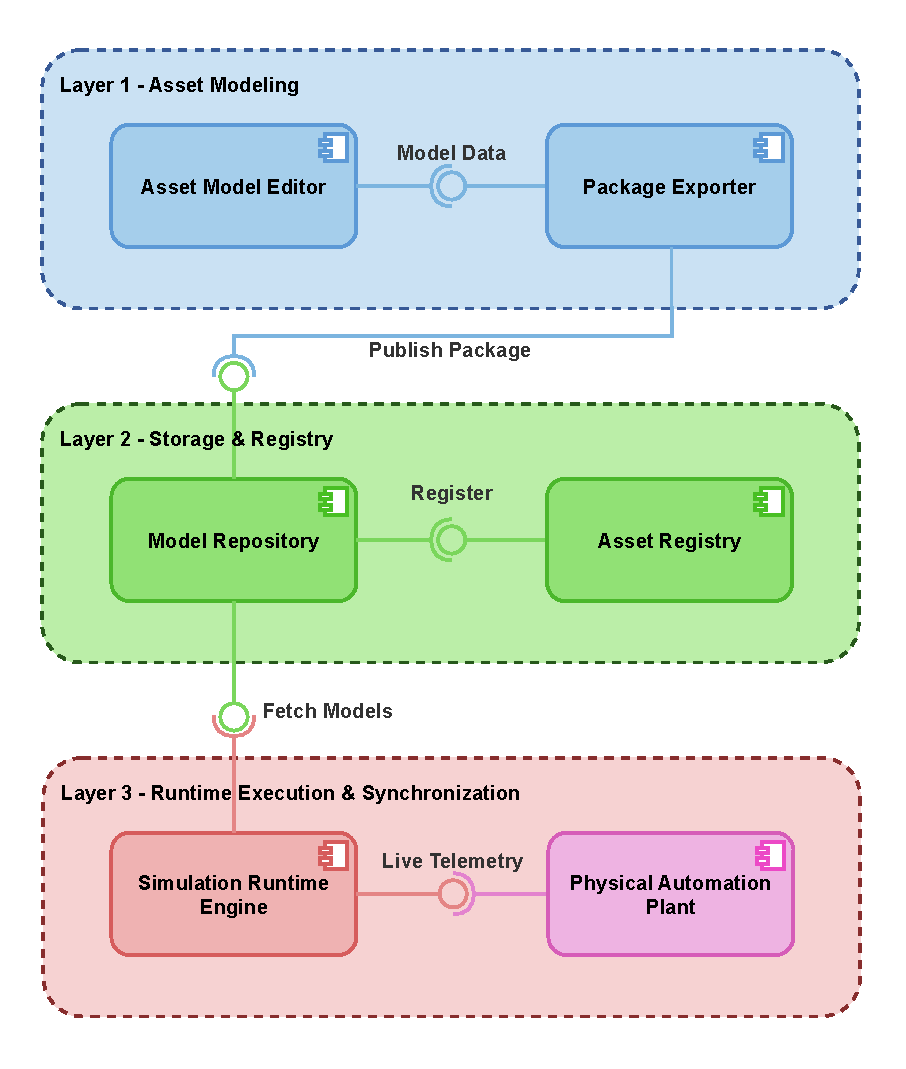
\includegraphics[width=\columnwidth]{figures/Arquitetura.drawio.pdf}
\caption{Conceptual architecture of the framework: asset modeling, storage and registry, and runtime execution layers. The optional digitization stage (Layer~0) is omitted.}
\label{fig:arch_conceptual}
\end{figure}

Layer~0, \textit{Physical Asset Digitization}, provides the geometric foundation. In greenfield projects, machine builders may supply lightweight, simulation-ready models, but real plants usually present one of two extremes: either no 3D model exists at all, or the only available model is a manufacturing CAD assembly. A raw CAD model of a stamping station, for instance, can contain hundreds of thousands of polygons in a static hierarchy without pivots or motion axes. Layer~0 therefore removes internal detail, decimates exterior surfaces, separates movable parts into independent sub-meshes whose local frames coincide with their physical axes of motion, and places invisible trigger volumes at the locations of the physical sensors. The result is exported as a self-contained file in an open binary 3D format. At this point the asset is geometrically correct but carries no automation data.

Layer~1, \textit{Asset Modeling}, turns this geometry into an operational asset description. In conventional workflows, sensors, actuators, and behaviors are configured inside a specific simulation suite, so that work is lost when the tool changes. Layer~1 keeps semantic modeling independent of any runtime engine. An engineer imports the Layer~0 model, assigns identity metadata, defines the kinematic properties of movable nodes, creates virtual pins that mirror the physical controller I/O points, attaches sensor pins to detection volumes and actuator pins to mechanisms, and optionally defines local control rules. The configuration is validated against the data model and compiled into a single immutable package that is published to Layer~2.

Layer~2, \textit{Storage and Registry}, is the discovery and distribution point of the ecosystem. Instead of locally copied model files and hard-coded addresses, Layer~2 separates heavy artifacts from lightweight metadata. A \textit{Model Repository} receives the packages, extracts their meshes and descriptors, and serves them over the Hypertext Transfer Protocol (HTTP), whereas an \textit{Asset Registry} records only identifiers, classifications, and endpoint URLs. Any authorized client can therefore discover which assets exist with one inexpensive query and download only what it needs.

Layer~3, \textit{Runtime Execution and Physical Synchronization}, produces and runs the virtual counterpart of the plant. The runtime queries Layer~2 at startup, downloads the packages of all registered assets, and reconstructs the scene in memory, creating visual nodes, physics colliders, kinematic controllers, and pin bindings from the descriptors. It then operates in one of two modes. In VC mode, the control sequences contained in the packages are evaluated locally and drive the virtual actuators, closing the loop entirely in software. In DT mode, the states reported by the controllers drive the virtual model, and the same sequences also dispatch commands to the controllers, which execute them on the real equipment. Because contact physics accumulates small numerical errors, physical sensor detections are treated as ground truth: when a hardware sensor confirms that a workpiece has reached a station, the virtual workpiece is moved to the known coordinates of that sensor, resetting the accumulated drift (FR4). After startup, the runtime keeps polling the registry, so that assets registered, removed, or relocated while it is running are added to, removed from, or rebuilt in the scene without restarting it.

\subsection{Cross-Layer Information Flows}
\label{sec:arch_flows}

Whereas some architectures serve 3D models and runtime signals from the same AAS server \cite{Pajpach2023}, the proposed architecture separates three information flows by lifecycle phase, payload size, and timing constraints.

The \textit{Asset Publication Flow} (design time, Layer~1 to Layer~2) occurs whenever an engineer creates or updates an asset. It carries large payloads, namely meshes and submodel descriptors packed into an archive, but it is not time-critical. The package is uploaded to the Model Repository and its identity and submodel endpoints are registered, after which the asset is immediately discoverable on the network. The \textit{Dynamic Ingestion Flow} (deployment time, Layer~2 to Layer~3) is triggered when a runtime instance starts or when a new asset enters the cell. The runtime first issues lightweight registry queries to learn which assets are present and then retrieves their geometry and submodels from the repository, so any asset registered in Layer~2 can be instantiated without re-engineering the application. The \textit{Telemetry Flow} (runtime, physical plant to Layer~3) runs continuously during production and is the only latency-critical one. It deliberately bypasses the storage and registry services: controllers send compact, event-driven state messages over a dedicated channel straight to the runtime, so that database access and large file transfers can never delay sensor events (NFR1).
\subsection{Asset Data Model}
\label{sec:arch_metamodel}

The asset data model is technology-neutral and describes each machine through a root entity and five submodel classes, shown in the Unified Modeling Language (UML) class diagram of Fig.~\ref{fig:arch_metamodel}. All attributes use primitive types (\textit{String}, \textit{Float}, \textit{Integer}, \textit{Boolean}) and \textit{Vector3}, a triple $(x, y, z)$ of floats.

\begin{figure*}[t]
\centering
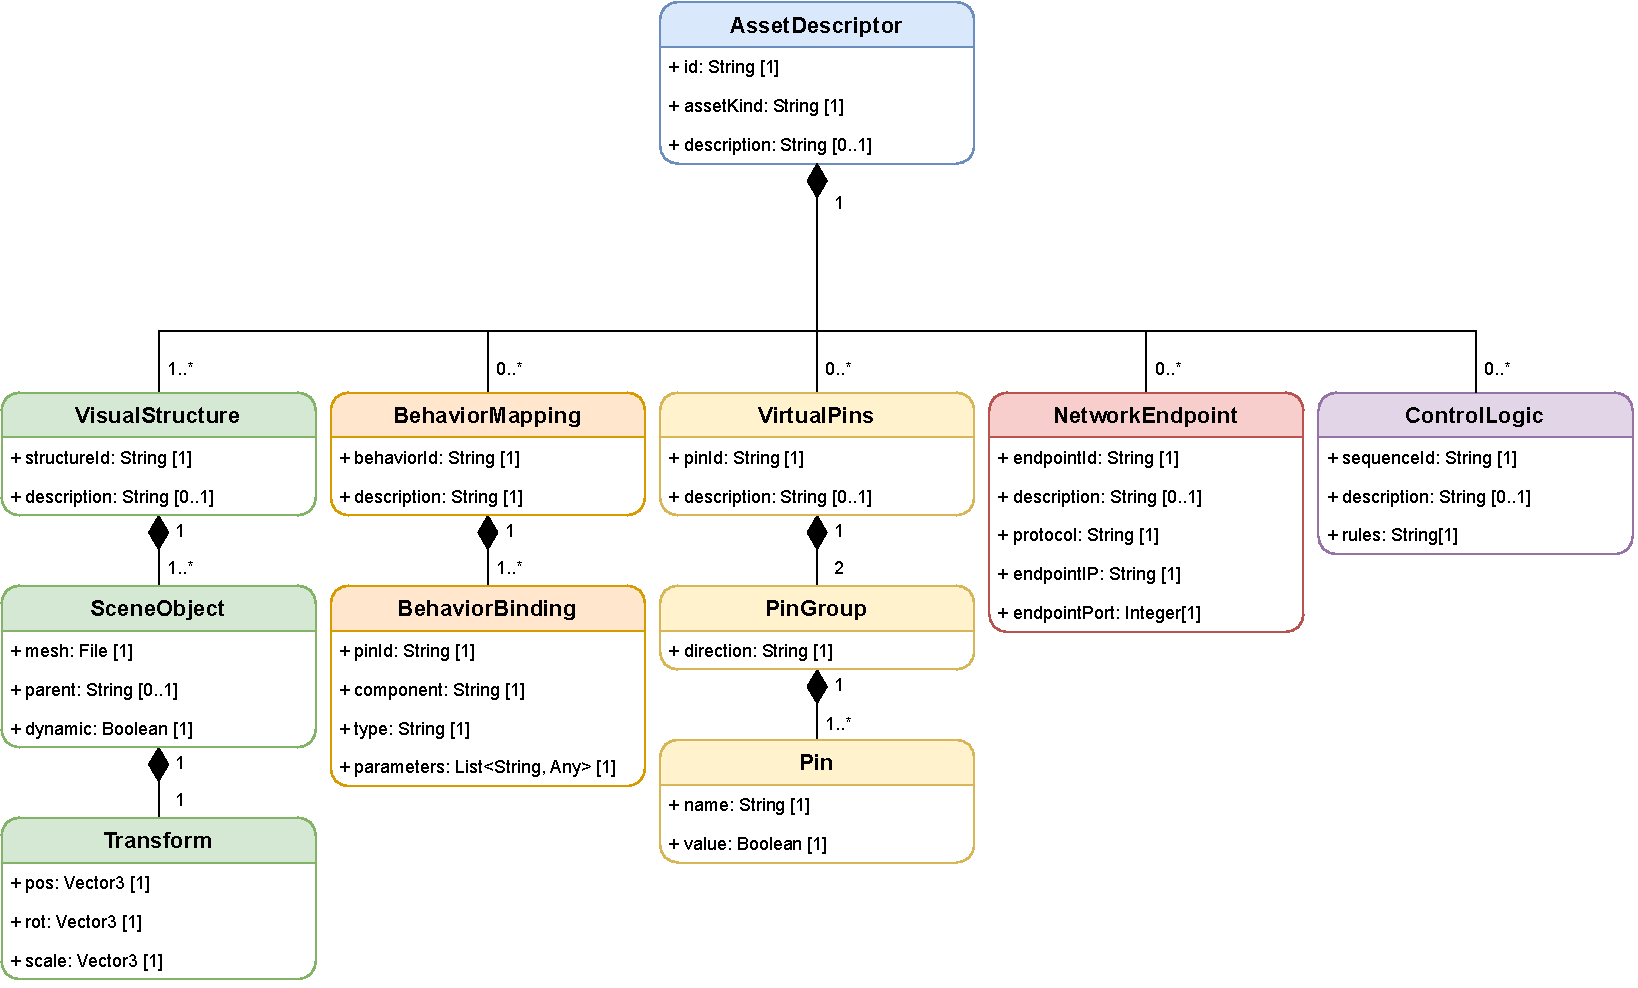
\includegraphics[width=0.92\textwidth]{figures/Modelo de Dados.drawio.pdf}
\caption{UML class diagram of the asset data model: the \textit{AssetDescriptor} root and its five submodel classes.}
\label{fig:arch_metamodel}
\end{figure*}

The \textit{AssetDescriptor} is the identity root of a machine or workstation. It holds a unique identifier, used for registry lookups and user interfaces, an asset kind distinguishing a type from a concrete instance, and an optional description. The mandatory \textit{VisualStructure} submodel describes the spatial composition of the asset independently of any graphics format. It contains one or more \textit{SceneObject} nodes, each referencing a mesh file, optionally naming a parent node to form multi-part assemblies, and flagging whether the part moves during operation. Every node carries one \textit{Transform}, with a position relative to its parent, Euler angles in degrees, and a scale vector that defaults to unity.

The optional \textit{BehaviorMapping} submodel bridges geometry and physics. It groups \textit{BehaviorBinding} entries that associate a pin identifier with a scene component and a mechanism type, together with an extensible parameter dictionary. Actuator mechanisms are \textit{Conveyor}, which imparts its surface velocity to the workpieces in contact with it, \textit{TranslateContinuous} and \textit{RotateContinuous} for unbounded motion, and \textit{TranslateFixed} and \textit{RotateHinge} for strokes between configurable limits. On the bench, the punch rod and the rotating platforms use continuous mechanisms whose end positions are detected by limit-switch sensors. Sensors use the \textit{TriggerZone} mechanism. For actuators, the parameters define a motion axis, a speed, the physical controller terminal (\textit{RealPortID}), and a flag that routes the actuator to real hardware. For sensors, they define a workpiece tag filter, the electrical polarity (\textit{ActiveLow}), the physical terminal, and a routing flag. Sensors may also carry a realignment specification consisting of the trigger edge (\textit{MoveOnState}), the scope of the correction (position, rotation, or both), and the ground-truth position and orientation to which a detected workpiece is moved. This specification is what enables drift correction in DT mode. Notably, \textit{BehaviorMapping} never stores signal values. These belong to the \textit{VirtualPins} submodel, the digital image of the controller registers, which organizes \textit{Pin} channels into an \textit{INPUT} group for sensor states coming from the plant and an \textit{OUTPUT} group for actuation commands, each pin holding a tag name and an instantaneous Boolean value.

The two remaining submodels describe behavior and connectivity. \textit{ControlLogic} stores a set of rule-triggered sequences, each with an identifier, a description, a trigger condition, and an ordered list of steps that the runtime executes when the trigger holds, which allows a cell to be exercised without any external PLC. \textit{NetworkEndpoint} specifies how the physical equipment is reached, namely a protocol (e.g., Transmission Control Protocol (TCP) socket or HTTP), an IP address or host name, and a port. Separating values (\textit{VirtualPins}) from their physical meaning (\textit{BehaviorMapping}) and from their transport (\textit{NetworkEndpoint}) is what allows the same package to drive both execution modes: only the source of the pin values changes when moving from VC to DT operation.

%=============================================================================
\section{Technological Implementation}
\label{sec:implementation}
%=============================================================================

The conceptual architecture was realized with open-source tools wherever possible and deployed against a physical conveyor bench. This section first gives an overview of the technology stack and the interfaces between layers, then details the implementation of each layer, and closes with the physical testbed and the embedded firmware that runs on its controller.

\subsection{Implementation Overview and Technology Stack}
\label{sec:impl_overview}

Fig.~\ref{fig:arch_implementation} shows the UML component diagram of the implementation. The choice of technologies followed three criteria: open standards at every interface, no dependency on proprietary simulation software, and the ability to run the whole stack on a single workstation. Layer~0 uses Blender~5.2 LTS and the glTF~2.0 binary format (GLB), which preserves node hierarchies, pivots, and materials in a single file and can be loaded at runtime by most engines. Layer~1 is a Python~3.10 desktop application built with PyQt6, PyVista/VTK, and Trimesh, and it relies on the official \texttt{basyx-python-sdk} so that the packages it produces are standard IEC~63278 AASX archives rather than a custom format. Layer~2 is the Eclipse BaSyx~v2 reference implementation, deployed with Docker Compose so that the full server stack can be reproduced with a single command. Layer~3 is implemented in Unity~6 (v6000.3.10f1) with C\#, using glTFast for runtime mesh import and the built-in PhysX engine for contact physics. On the plant side, an Industrial Shields M-DUINO PLC runs custom FreeRTOS firmware.

\begin{figure}[t]
\centering
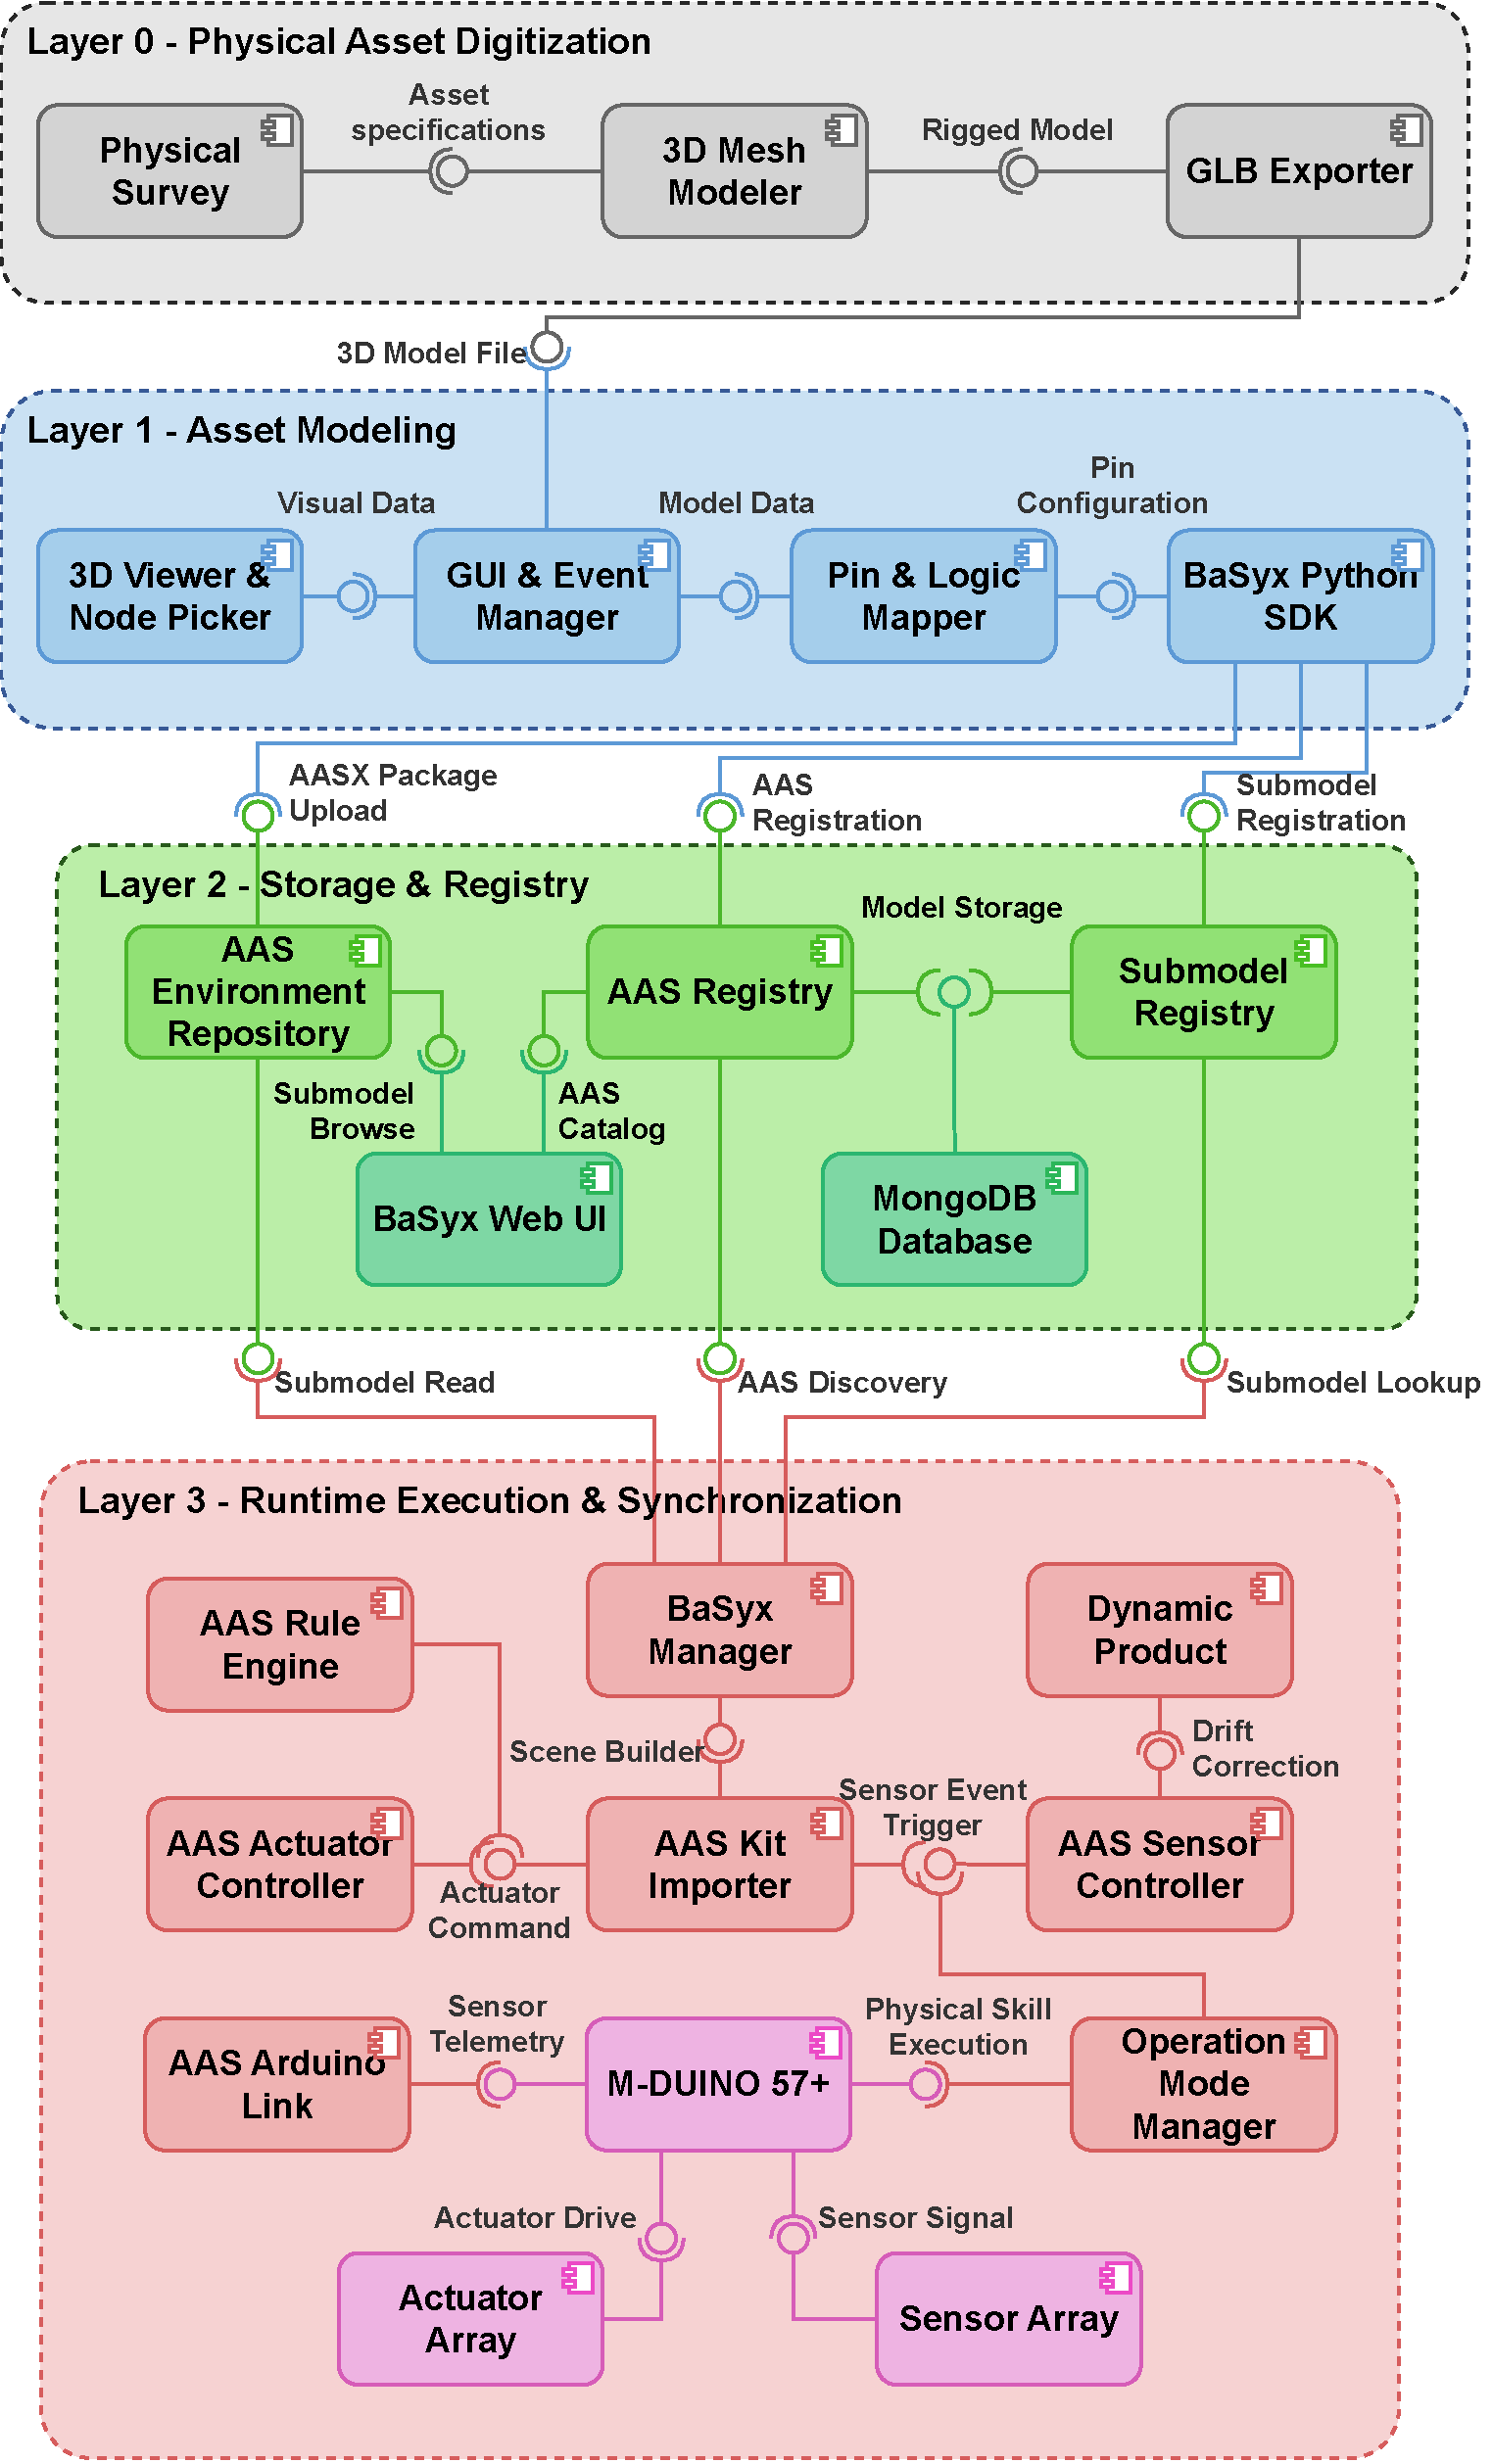
\includegraphics[width=\columnwidth]{figures/Implementacao_paper.drawio.pdf}
\caption{UML component diagram of the implementation: (0) digitization in Blender, (1) asset modeling in the Python application, (2) storage and registry in Eclipse BaSyx~v2 on Docker, and (3) runtime execution in Unity~3D connected to an Industrial Shields M-DUINO PLC.}
\label{fig:arch_implementation}
\end{figure}

The layers interact through four interfaces only. A GLB file is passed from Layer~0 to Layer~1. An AASX package is uploaded from Layer~1 to Layer~2 through an HTTP POST request. Layer~3 reads registry descriptors, submodels, and mesh files from Layer~2 through HTTP GET requests. Finally, the runtime and the PLC exchange state over a raw TCP socket (port~8888) for telemetry and an HTTP server (port~80) for commands. Because each interface is a file or a standard network API, any layer can be replaced, restarted, or scaled without modifying the others, which is the practical meaning of NFR3.

\subsection{Layer 0: Physical Asset Digitization}
\label{sec:impl_layer0}

Because the modular bench used in this work came without vendor 3D models, Layer~0 was carried out manually in Blender. Each module was measured on the physical bench and rebuilt at a 1:1 metric scale (one Blender unit equal to one meter), matching Unity's unit convention so that no rescaling is needed downstream. Each asset was organized as a clean parent--child hierarchy. Static frame parts were merged into a single root node with its origin at the base reference point $(0,0,0)$, whereas dynamic elements, such as belt surfaces, rotating platforms, and the punch rod, were isolated as child objects. The pivot of every dynamic child was then aligned with its physical axis of rotation or translation; a misplaced pivot would make the part orbit or slide along an unintended path when driven by a \textit{BehaviorBinding} at runtime. Finally, invisible trigger volumes were placed at the positions of the physical sensors and the assets were exported as GLB files. Fig.~\ref{fig:fms_vs_blender} compares a physical module with its reconstruction.

\begin{figure}[t]
\centering
\subfloat[Physical conveyor module.\label{fig:fms_physical}]{%
  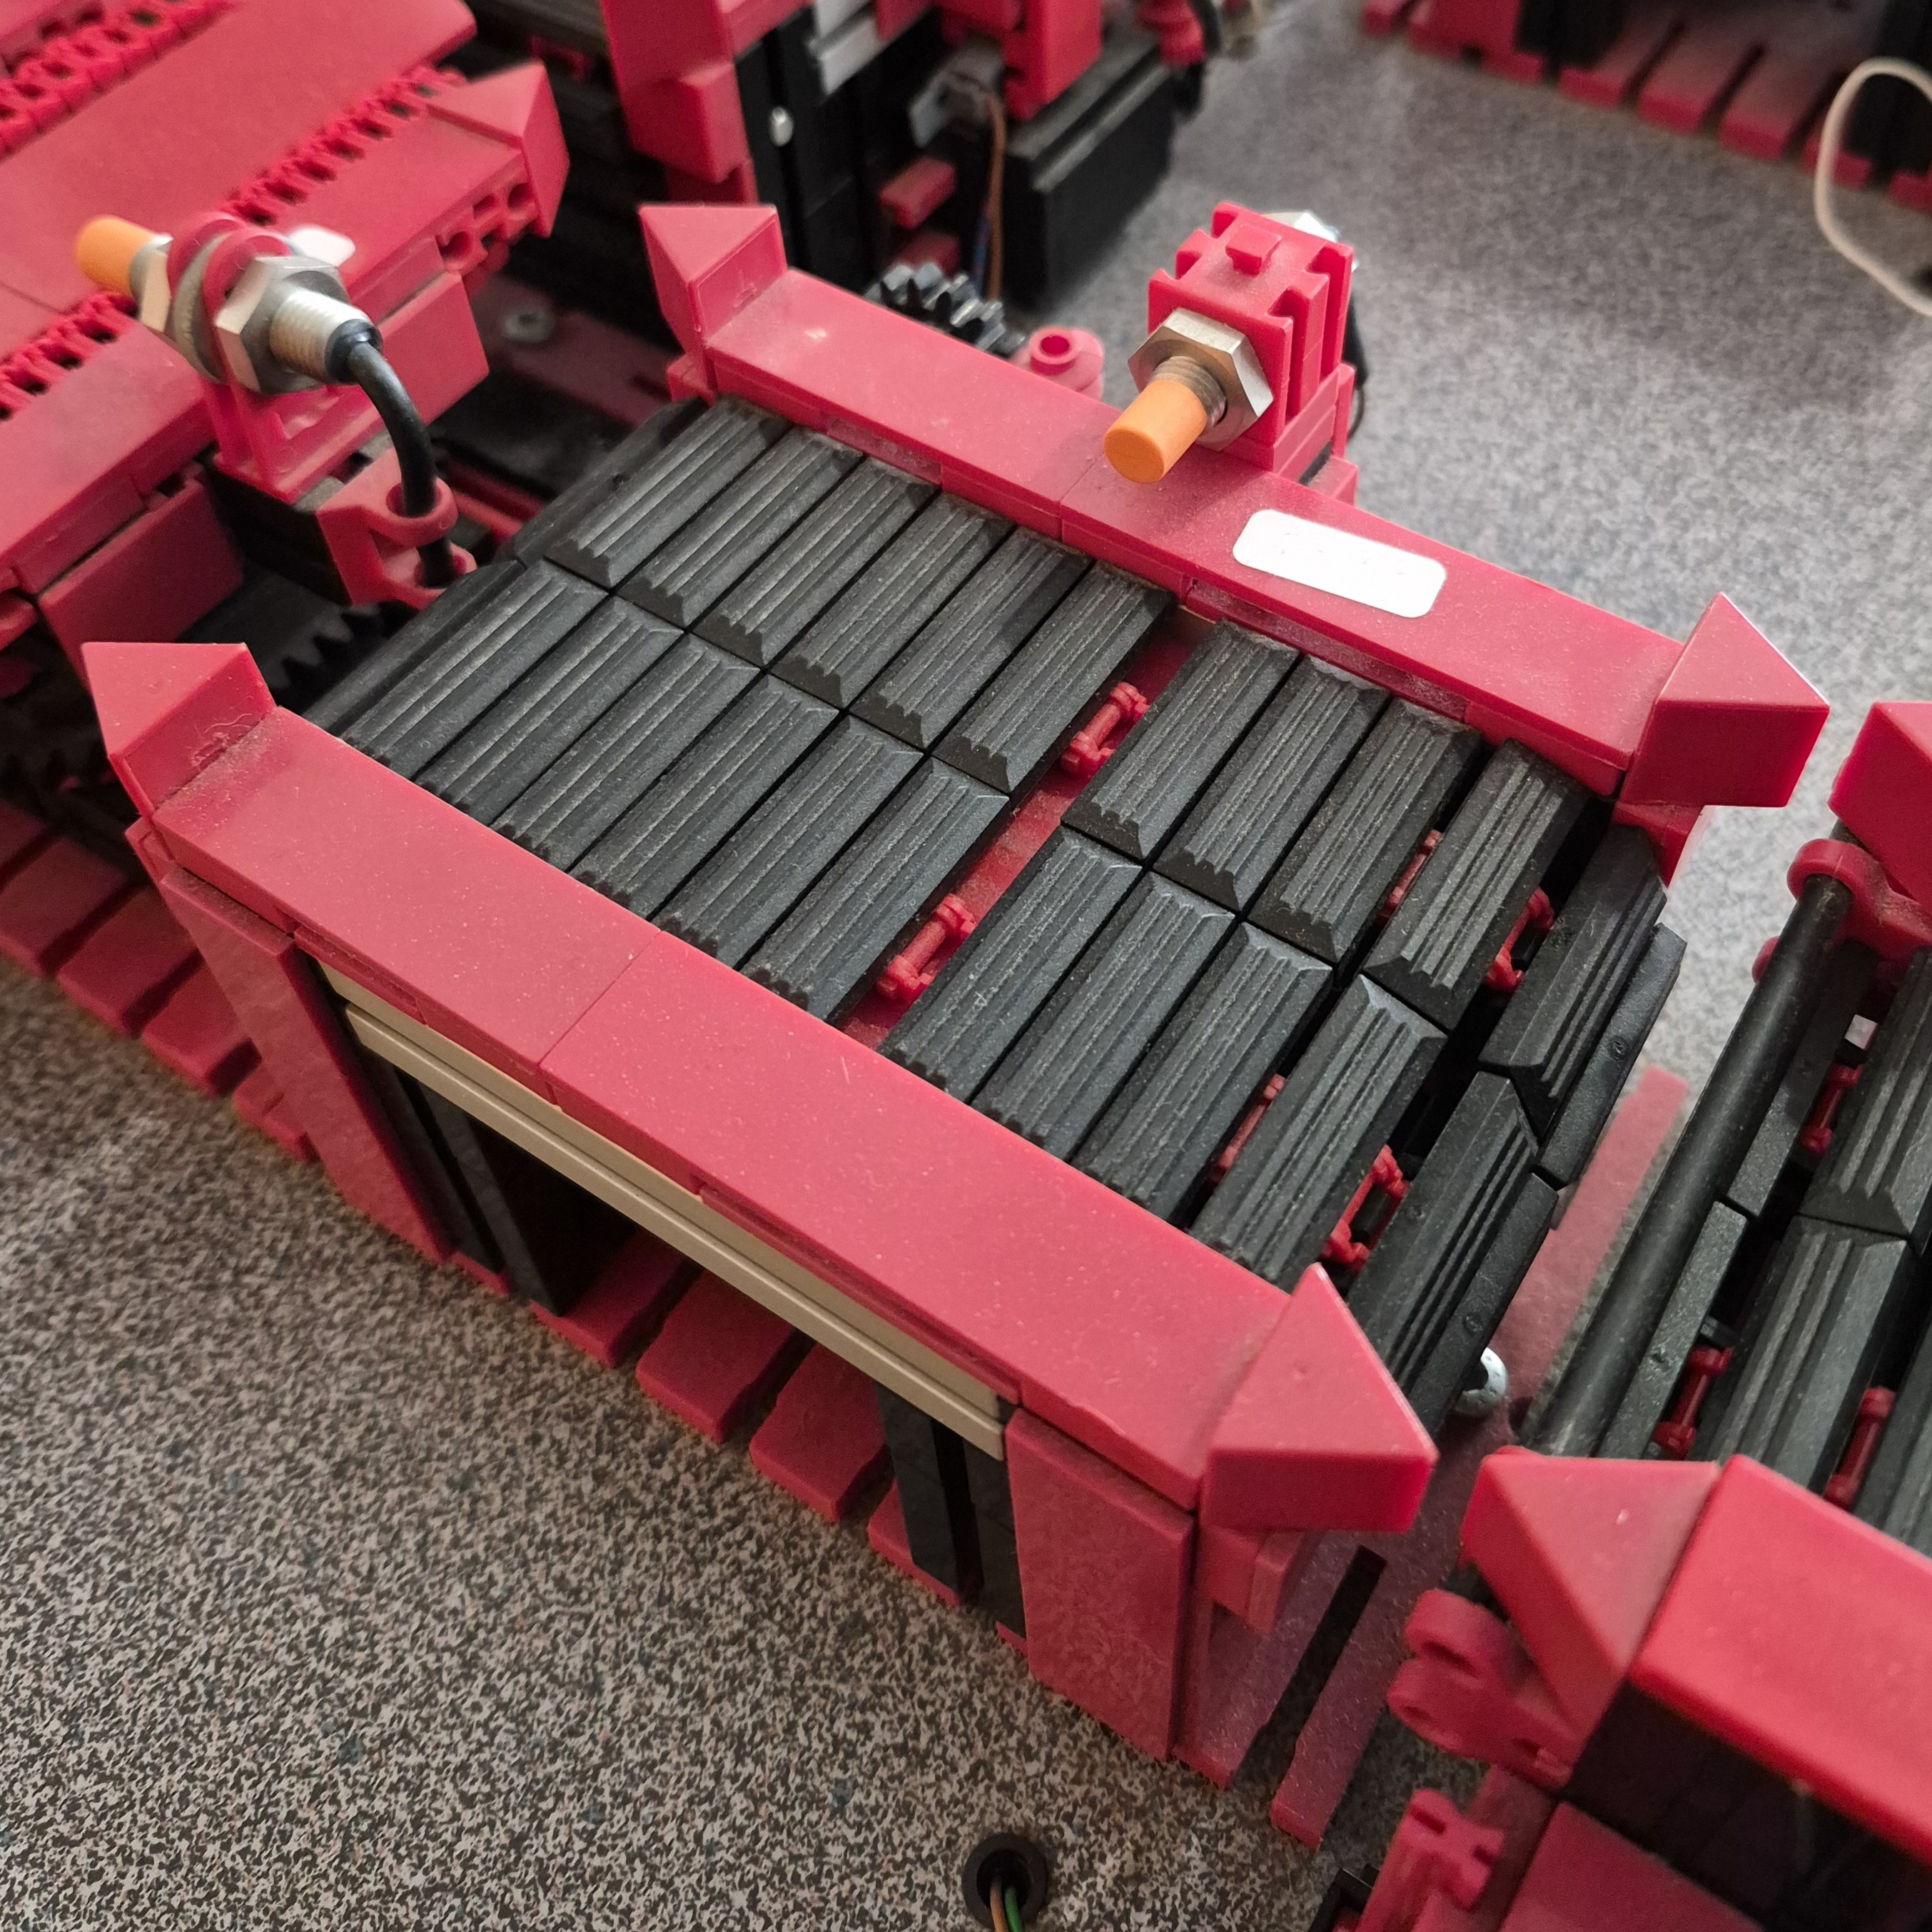
\includegraphics[width=0.48\linewidth,height=3.4cm,keepaspectratio]{figures/fms_conveyor_sensors_closeup.jpg}%
}\hfill
\subfloat[Reconstructed 3D asset.\label{fig:fms_blender}]{%
  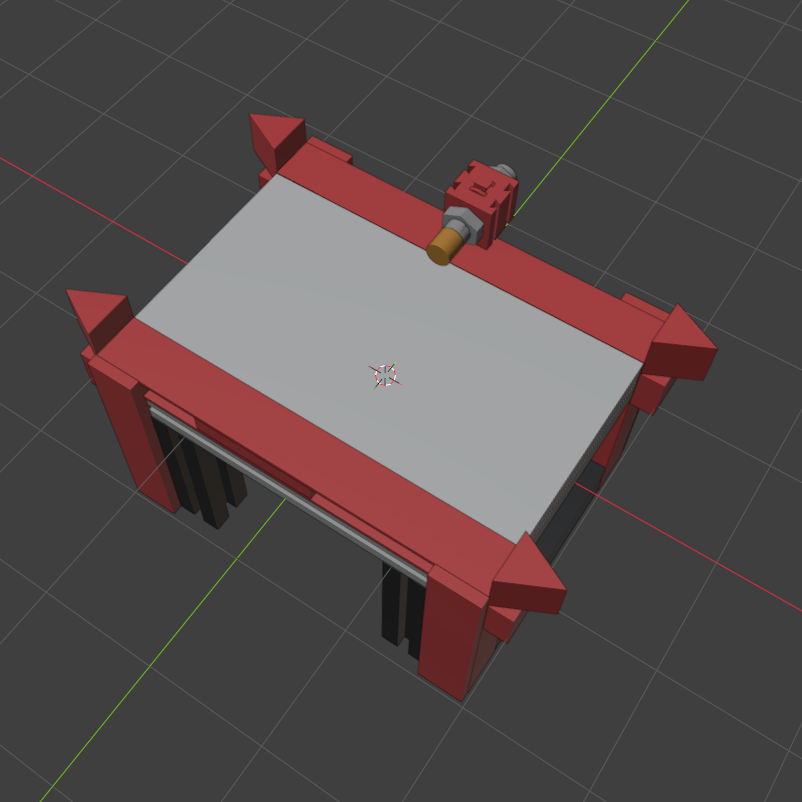
\includegraphics[width=0.48\linewidth,height=3.4cm,keepaspectratio]{figures/blender_kLfhitpziL.png}%
}
\caption{Physical FMS conveyor module and its low-polygon, rigged reconstruction in Blender (Layer~0).}
\label{fig:fms_vs_blender}
\end{figure}

% Defined here (before its first citation) so that, as a two-column float,
% it lands at the top of the next page, close to Section IV-C.
\begin{figure*}[t]
\centering
\subfloat[Wizard (step 2) and 3D viewport.\label{fig:asset_modeling_gui}]{%
  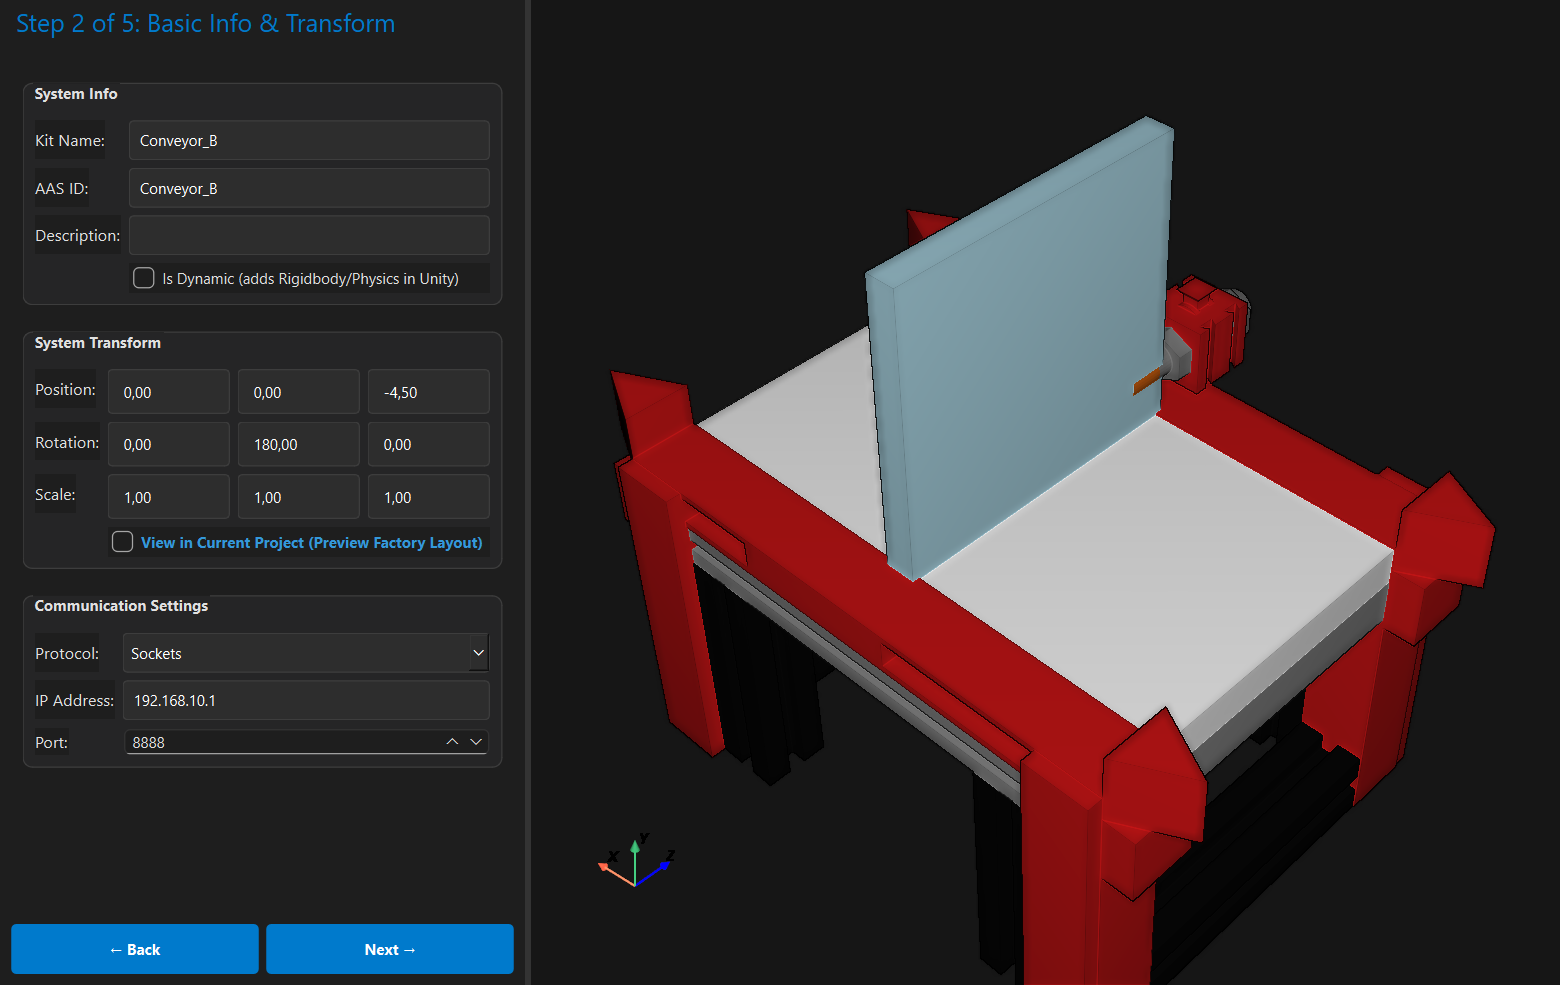
\includegraphics[height=5cm]{figures/paper_l1_wizard_crop.png}%
}\hfill
\subfloat[Sensor configuration.\label{fig:case_study_step2_sensors}]{%
  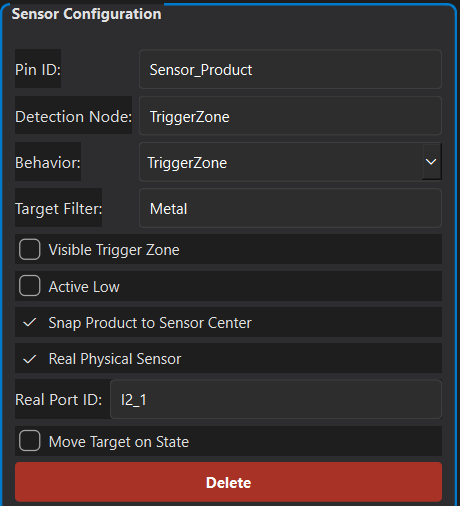
\includegraphics[height=5cm]{figures/paper_l1_sensors_crop.png}%
}\hfill
\subfloat[Actuator configuration.\label{fig:case_study_step2_actuators}]{%
  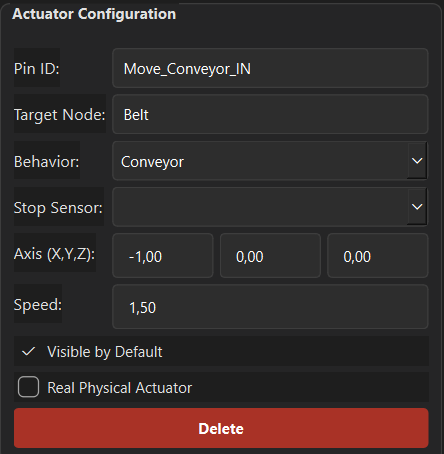
\includegraphics[height=5cm]{figures/paper_l1_actuators_crop.png}%
}
\par\vspace{1mm}
\subfloat[No-code \textit{ControlLogic} rule editor with the A$\rightarrow$B transfer sequence.\label{fig:rule_editor_gui}]{%
  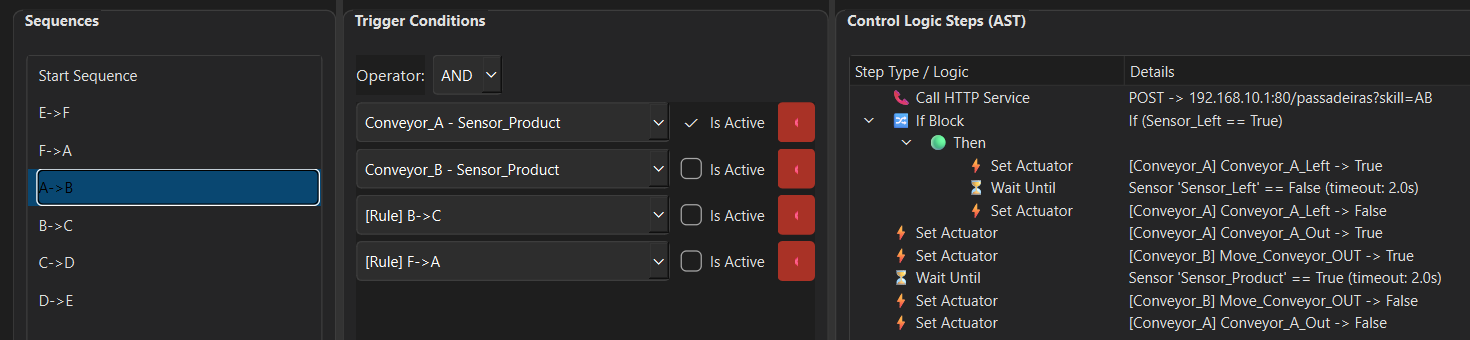
\includegraphics[width=\textwidth]{figures/paper_l1_rules_crop.png}%
}
\caption{Layer~1 asset modeling application, (a)~identity, placement, and network endpoint of Conveyor~B, (b)--(c)~virtual pin configuration of Conveyor~F, and (d)~rule editor.}
\label{fig:layer1_gui}
\end{figure*}

\subsection{Layer 1: Asset Modeling Application}
\label{sec:impl_wizard}

Layer~1 merges the asset model editor and the package exporter of the conceptual architecture into a single desktop application (Fig.~\ref{fig:asset_modeling_gui}). Its interface has three regions: a central PyVista/VTK viewport with orbit and pan controls and markers for placed pins and coordinate axes, a left-hand wizard that guides the engineer through five steps, and a right-hand tree, omitted from Fig.~\ref{fig:asset_modeling_gui} for legibility, that exposes the node hierarchy of the imported model. In the first step, the engineer loads the GLB file, whose hierarchy and bounding dimensions are verified with Trimesh. The second step collects the identity metadata (AAS identifier, name, description), the placement of the asset in the cell, and its network endpoint. In Fig.~\ref{fig:asset_modeling_gui}, for instance, Conveyor~B is placed at $(0, 0, -4.5)$ with a $180^\circ$ rotation about the vertical axis and is reached through a socket connection to the PLC at port~8888. The light-blue box in the viewport is the trigger volume modeled in Layer~0. The third and fourth steps configure sensors and actuators, and the fifth step displays the resulting submodel tree and JSON manifest before export and upload.

Sensor configuration is the step in which manual workflows are most error-prone, so the application never asks for coordinates. Instead, each sensor pin is attached by name to one of the detection volumes modeled in Layer~0 (Fig.~\ref{fig:case_study_step2_sensors}). In the example, the pin \texttt{Sensor\_Product} is bound to the \texttt{TriggerZone} node with the \textit{TriggerZone} mechanism and reacts only to workpieces tagged \texttt{Metal}. The same form sets the electrical polarity (\textit{Active Low}), routes the pin to a real PLC input (here \texttt{I2\_1}), and defines the realignment specification used for drift correction: \textit{Snap Product to Sensor Center} moves a detected workpiece to the sensor position, and \textit{Move Target on State} selects the triggering edge. Actuators are configured in a similar way (Fig.~\ref{fig:case_study_step2_actuators}). The pin \texttt{Move\_Conveyor\_IN} drives the \texttt{Belt} sub-mesh with the \textit{Conveyor} mechanism along the axis $(-1, 0, 0)$ with a configured surface speed, and an optional stop sensor can halt it when a workpiece arrives. Because its \textit{Real Physical Actuator} flag is cleared, this pin acts only on the virtual model. Flagged pins are additionally bound to a relay output of the PLC.

To support stand-alone VC, the application also includes a no-code \textit{ControlLogic} editor (Fig.~\ref{fig:rule_editor_gui}). Engineers compose sequences from nine block types: setting an actuator, waiting for a fixed time, waiting until a sensor condition holds,\textit{If/Then} and \textit{If/Else} branches, \textit{While} loops, fixed repetitions, internal variable assignments, and outbound HTTP calls that can trigger external services or physical controllers. Each sequence is started by a set of \textit{trigger conditions} combined with an AND or OR operator. A condition refers either to a sensor pin of any asset in the cell or to another sequence, and requires it to be active or inactive. This allows sequences that share equipment to interlock without explicit locking code. The A$\rightarrow$B transfer in Fig.~\ref{fig:rule_editor_gui}, for example, starts only when a workpiece is present on Conveyor~A, Conveyor~B is free, and neither the B$\rightarrow$C nor the F$\rightarrow$A sequence is running. Its steps then notify the PLC through an HTTP call, drive the belts of both conveyors, wait until \texttt{Sensor\_Product} on Conveyor~B detects the workpiece, and stop both belts. The rule engine evaluates the triggers of all idle sequences every 100\,ms. The sequences are stored as an abstract syntax tree in the \textit{ControlLogic} submodel.Once all information is defined, the application builds the AASX package in memory with \texttt{basyx-python-sdk}, embedding the GLB mesh as a supplementary file referenced by a \textit{File} element and serializing the submodels as standard-compliant JSON, and uploads it to the Layer~2 repository. \textit{ControlLogic} is included only when the asset carries sequences, and \textit{NetworkEndpoint} is serialized under the identifier \textit{AssetInterfacesDescription}.

\subsection{Layer 2: Storage and Registry}
\label{sec:impl_basyx}

Layer~2 is the Eclipse BaSyx~v2 stack orchestrated with Docker Compose. The AAS Environment Repository (port~8081) receives AASX packages, extracts embedded files so that meshes become available at stable URLs, and exposes shells and submodels through the standard REST API. The AAS Registry (port~8082) and the Submodel Registry (port~8083) maintain lightweight directories that map identifiers to endpoint URLs, MongoDB (port~27017) persists descriptors and submodels, and the BaSyx Web UI (port~3000) lets operators inspect the registered assets. When a package is uploaded, the repository decompresses the archive, stores its submodels, and registers the shell and submodel descriptors, after which a single \texttt{GET /shell-descriptors} request to the registry is enough for a client to enumerate all active machines. Because storage and discovery are independent services, additional repositories or registry replicas can be added as the number of assets and clients grows (NFR2). The MQTT and InfluxDB services of the standard BaSyx deployment are deliberately left out of the telemetry path (Section~\ref{sec:arch_flows}).

\subsection{Layer 3: Runtime Execution and Physical Synchronization}
\label{sec:impl_unity}

The Unity runtime contains no pre-built factory scene, and everything it displays is built from Layer~2 at launch in three phases. In the discovery phase, the orchestrator clears cached files from previous sessions, waits until the registry is reachable, and retrieves all shell descriptors with a single \texttt{GET /shell-descriptors} request. It then starts one ingestion coroutine per shell.

In the construction phase, each coroutine resolves the identifiers of the asset's submodels, resets its \textit{VirtualPins} to a safe state, reads \textit{VisualStructure} and the network endpoint, and downloads every \textit{File} element, i.e., the GLB meshes, through the \texttt{/attachment} endpoint of the repository into a local cache. The runtime therefore never handles AASX archives, which the repository unpacks at upload time. Static equipment is built first, whereas workpieces, flagged as dynamic in \textit{VisualStructure}, are spawned only after a settling delay so that they cannot fall through colliders that are still being created. The node hierarchy of each asset is rebuilt in memory with glTFast, which converts the right-handed glTF frame to Unity's left-handed one. Non-uniform scales are applied to vertices to avoid distorted child transforms, and convex mesh colliders and kinematic rigid bodies are attached to the reconstructed nodes. The importer then parses \textit{VirtualPins} and \textit{BehaviorMapping}, creating sensor trigger volumes at the authored positions and attaching motion controllers to the actuated parts. Control sequences are staged during construction and started only once every asset exists, so that no sequence refers to a component that has not yet been created.

In the execution phase, after a short settling period for the physics engine, the runtime enters one of its two modes. From then on, a discovery loop queries the registry every 2\,s. Newly registered shells are ingested, deregistered ones are destroyed, and every instantiated asset compares its \textit{VisualStructure} with the repository at the same rate and rebuilds itself when, for instance, its placement changes. All ingestion coroutines are interleaved on Unity's main thread and advance at most one step per rendered frame. This keeps the scene responsive while assets are loading, but it couples ingestion time to frame time, as discussed in Section~\ref{sec:res_stress_testing}.

Conveyors are simulated through contact physics: an active belt imposes its surface velocity on the workpieces it touches, and PhysX resolves gravity and contacts in the 50\,Hz fixed-step loop, so that transfers, blockages, and collisions emerge from the layout instead of being scripted. In VC mode, the rule engine loads the sequences from \textit{ControlLogic} and evaluates their trigger conditions every 100\,ms against the states of the virtual sensors. The steps of a triggered sequence drive the virtual actuators, and calls to external services are skipped, so the loop is closed entirely in software. In DT mode, the runtime starts one background thread per controller endpoint declared in \textit{NetworkEndpoint}. Each thread keeps a TCP connection to port~8888 of the PLC, parses the incoming JSON state messages, and pushes them into a concurrent queue. Unity's main thread drains this queue once per frame and dispatches every change to the sensor and actuator controllers subscribed to that terminal, so that actuators flagged as real follow the relay states reported by the PLC instead of local commands. The opposite direction, from twin to plant, is closed by the same sequences used in VC. In DT mode, a sequence starts when its trigger holds either in the simulation or on the physical sensors, and its HTTP steps are sent to the command server of the PLC on port~80 (e.g., \texttt{/passadeiras?skill=AB} in Fig.~\ref{fig:rule_editor_gui}), which executes the corresponding transfer on the real bench. The remaining steps are mirrored in the simulation, and wait steps are released by whichever sensor, virtual or physical, confirms the event first. Sensor changes detected in the scene are also written back to \textit{VirtualPins} through asynchronous HTTP PUT requests.

Drift correction relies on the realignment data authored in Layer~1 and is applied at two moments. At startup in DT mode, the runtime waits for the initial burst of telemetry in which the PLC reports the state of all inputs. It then moves kinematic parts to the positions implied by the active sensors, for example a rotating conveyor to its end position, and snaps a workpiece onto every active sensor that carries a realignment specification, so that the twin starts from the actual state of the plant. During operation, whenever a sequence waits for a sensor and the physical sensor confirms the event, the workpiece is moved to the ground-truth coordinates of that sensor. At startup and in VC mode, a snap is applied only when the deviation exceeds a small position or orientation tolerance. Besides the pose, it clears the velocities accumulated by the solver. Since every transfer ends at a sensor, the position error of a workpiece is reset at each station and cannot accumulate over cycles. In VC mode, the same specification centers a workpiece when it enters a virtual sensor volume.

\subsection{Physical Testbed and Embedded Firmware}
\label{sec:impl_testbed}

The framework was deployed on an existing modular FMS bench (Fig.~\ref{fig:fms_pilot_testbed}) built following the modular CPPS principles of Rocha \etal \cite{Rocha2024}. The bench is assembled from \textit{fischertechnik} mechatronic modules arranged as a closed-loop conveyor circuit that transports workpieces between stations. It comprises three stationary linear conveyors (B, D, and F), two rotating conveyors (C and E), one translating conveyor (A), and a punch station that emulates stamping or drilling operations. Its field instrumentation consists of 24\,V~DC magnetic sensors that detect workpieces along the tracks, push-button limit switches that detect the end positions of the moving conveyors and the punch, and 24\,V~DC motors driving each section. Control is performed by an Industrial Shields M-DUINO 57R+ PLC, based on the ATmega2560 microcontroller with a W5500 Ethernet controller and optocoupled I/O, which reads sensors on digital inputs \texttt{I0\_0}--\texttt{I2\_5} and drives motors and the punch through relay outputs \texttt{R0\_2}--\texttt{R2\_8}.

\begin{figure}[t]
\centering
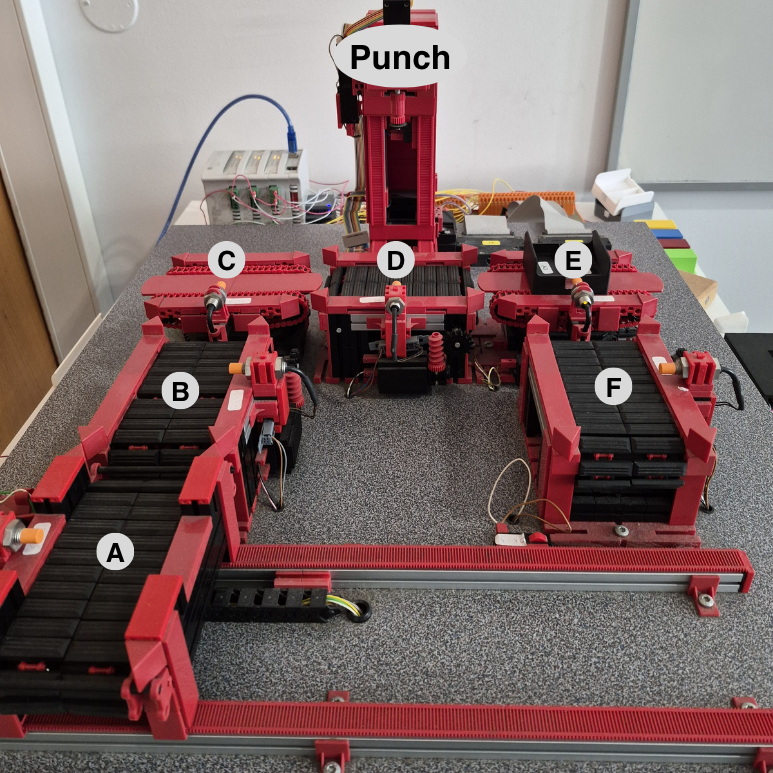
\includegraphics[width=0.85\linewidth]{figures/fms_pilot_bench.jpg}
\caption{Physical modular FMS conveyor bench with linear, rotating, and translating conveyors, punch station, and Industrial Shields M-DUINO PLC.}
\label{fig:fms_pilot_testbed}
\end{figure}

The PLC runs embedded firmware on the Arduino port of the FreeRTOS real-time operating system, which realizes the plant side of the telemetry and command channels defined in the architecture through four concurrent tasks. To protect the 5\,V logic from the electrical noise caused by motor switching, all field inputs pass through optocoupled galvanic isolation stages. The sensor task scans the 18 digital inputs once per scheduler tick, about 15\,ms with the default watchdog-based tick of this port, and compares each reading with the last transmitted value. Each state transition, as well as each change of the relay outputs, is placed in a 30-element first-in, first-out (FIFO) queue, so that network bandwidth is consumed by events rather than by cyclic polling and short periods of network congestion do not cause transitions to be lost. The telemetry task blocks on this queue and, as soon as an event arrives, serializes it as a compact JSON message containing the port identifier and its new value and streams it over the TCP socket on port~8888 to the runtime (NFR1). A command task hosts an HTTP server on port~80 through which the DT or any external client requests \textit{skills} from the bench, such as transferring a workpiece between two conveyors. The start of each skill is also reported over the telemetry channel. Finally, a connection monitor task manages the session with the runtime: it accepts the TCP connection and detects disconnections. Whenever a client reconnects, it clears the cached input states, so that the next scan retransmits the state of all inputs and the twin restarts from a consistent snapshot without interrupting the automation routines.

%=============================================================================
\section{Experimental Evaluation}
\label{sec:results}
%=============================================================================

The framework was evaluated through a case study of asset onboarding, a benchmark on the replica of the physical bench, a parametric stress test, and an analysis of the telemetry path in DT mode. All performance runs were executed in VC mode, which exercises the complete runtime (ingestion, contact physics, sensor callbacks, and rule engine) without its timing being bounded by the PLC. All measurements were taken on a workstation with an Intel Core i7-13650HX central processing unit (CPU) (14 cores, 20 threads, up to 4.9\,GHz), 16\,GB of DDR5 RAM, and an NVIDIA GeForce RTX~4060 Laptop GPU (8\,GB), running Windows~11 and Unity~6 (v6000.3.10f1).

\subsection{Case Study: End-to-End Asset Onboarding}
\label{sec:res_case_study}

To assess the authoring workflow (NFR4) and plug-and-play onboarding (FR1), an additional conveyor module, \textit{Conveyor~G}, was introduced into the cell. Conveyor~G has no physical counterpart: it represents a planned extension of the line, the situation in which VC is used to evaluate a layout change before hardware is installed. It was modeled in Blender after the existing linear conveyors, with the belt separated from the static frame, and exported as \texttt{Conveyor\_G.glb}. In the asset modeling application, following the procedure of Fig.~\ref{fig:case_study_step2_sensors}--\ref{fig:case_study_step2_actuators}, a presence sensor was attached to the trigger volume of the belt and a belt actuator was bound to the belt sub-mesh. Since the module is virtual, neither pin was flagged as routed to hardware. A transfer sequence from Conveyor~A to Conveyor~G was then defined in the rule editor in the same way as the A$\rightarrow$B sequence of Fig.~\ref{fig:rule_editor_gui}, triggered by the presence sensor of Conveyor~A and ending when the presence sensor of Conveyor~G detects the workpiece. The tool compiled the package and uploaded it to BaSyx, where the Web UI confirmed the registration of the \textit{VisualStructure}, \textit{BehaviorMapping}, \textit{VirtualPins}, and \textit{AssetInterfacesDescription} (network endpoint) submodels of Conveyor~G.

The runtime was already executing the cell, and no scene had been prepared for the new module. In its next discovery cycle, the runtime found Conveyor~G in the registry, downloaded its mesh and submodels, and instantiated its hierarchy, colliders, and pin bindings, while the rest of the cell kept running (Fig.~\ref{fig:case_study_step4}). The geometry and pins of a new asset therefore join a running scene within one discovery cycle. Its control sequences do not: because the rule engine reads \textit{ControlLogic} when it is initialized, the new A$\rightarrow$G sequence became active only after the scene was reloaded, which takes about 3\,s (Section~\ref{sec:res_fms_bench}) and requires no recompilation.
\begin{figure}[t]
\centering
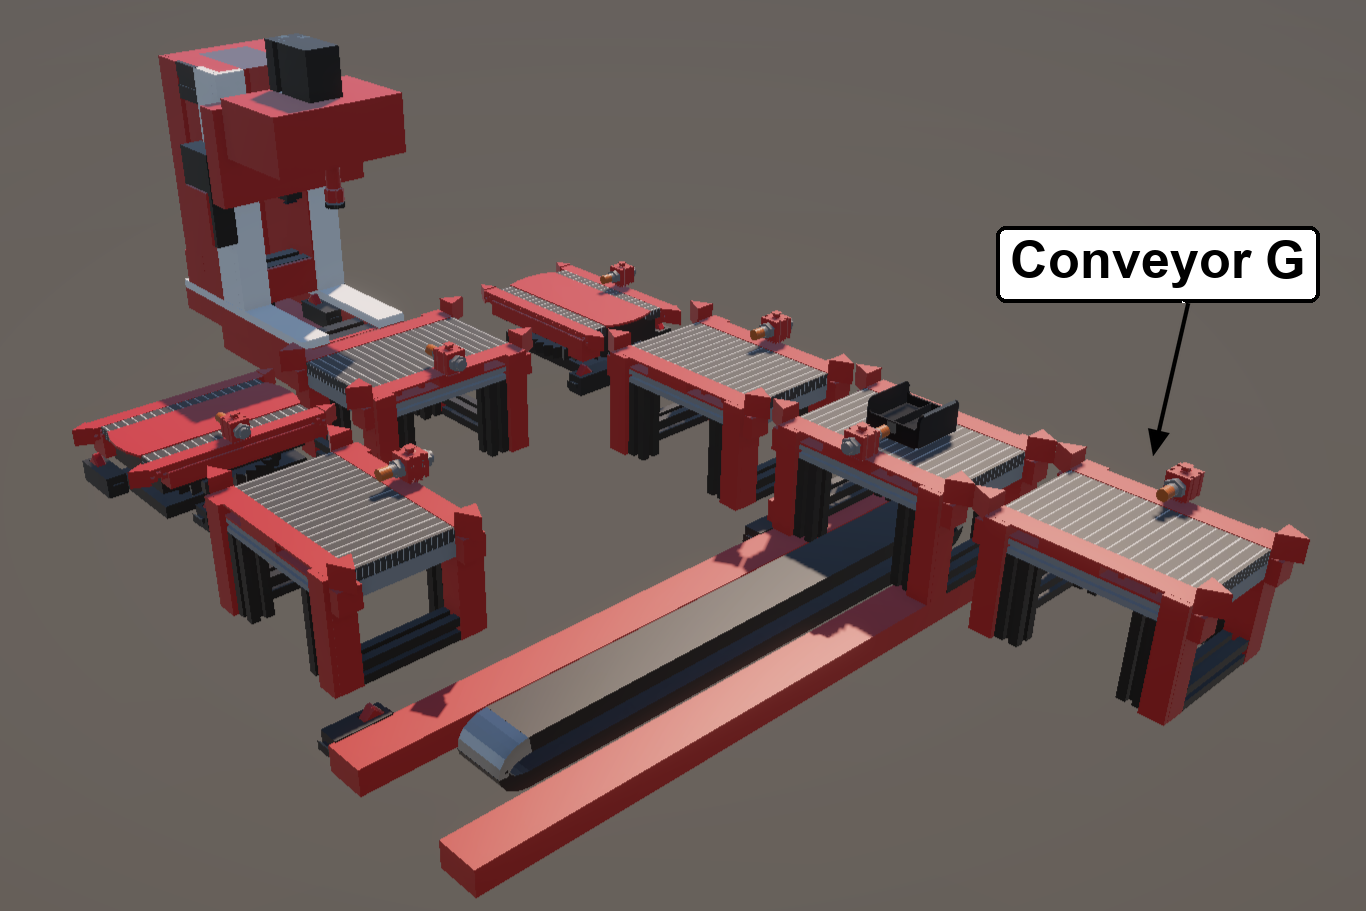
\includegraphics[width=\linewidth]{figures/5-unity_annotated.png}
\caption{Procedurally assembled scene in Unity~3D. Conveyor~G (marked) was instantiated from its AASX package without modifying the scene.}
\label{fig:case_study_step4}
\end{figure}

\subsection{Pilot Bench Performance}
\label{sec:res_fms_bench}

The virtual replica contains all modules of the physical bench (three linear, two rotating, and one translating conveyor, plus the punch station) with their sensor volumes and actuators. An automated harness performed 100 independent cold starts, each one retrieving the asset descriptors and meshes from BaSyx, building kinematics and friction physics, binding sensor callbacks, and executing the simulation. From frame durations sampled every 500\,ms in steady state, four metrics were derived: the mean frame rate in frames per second (FPS), i.e., the average of the inverses of the sampled frame durations, compared with the 60\,FPS (16.6\,ms) target for fluid interaction and the 30\,FPS minimum below which stutter becomes noticeable; the mean frame time; the \textit{1\% low} frame rate, i.e., the 1st percentile of the sampled frame rates, which reveals transient stalls; and the 95th and 99th percentile (P95, P99) frame times. Table~\ref{tab:fms_results} summarizes the results.

\begin{table}[t]
\centering
\caption{Pilot Bench Performance Across 100 Cold-Start Runs.}
\label{tab:fms_results}
\renewcommand{\arraystretch}{1.25}
\begin{tabular*}{\columnwidth}{@{\extracolsep{\fill}}lrrr@{}}
\toprule
\textbf{Metric} & \textbf{Mean $\pm$ Std} & \textbf{Min} & \textbf{Max} \\
\midrule
Startup time (s)        & $2.79 \pm 0.04$    & $2.72$   & $2.96$   \\
Mean frame rate (FPS)   & $489.91 \pm 49.21$ & $352.66$ & $694.09$ \\
1\% low frame rate (FPS)& $272.43 \pm 87.32$ & $104.60$ & $414.18$ \\
Mean frame time (ms)    & $2.36 \pm 0.39$    & $1.56$   & $3.91$   \\
P95 frame time (ms)     & $3.84 \pm 1.47$    & $2.38$   & $8.53$   \\
P99 frame time (ms)     & $4.35 \pm 2.01$    & $2.41$   & $9.94$   \\
\bottomrule
\end{tabular*}
\end{table}

Procedural instantiation of the complete bench took $2.79$\,s on average with a standard deviation of only $0.04$\,s, with an interquartile range between $2.76$ and $2.80$\,s, which indicates that descriptor retrieval and collider generation behave deterministically across cold starts. In steady state, the simulation ran at $489.91$\,FPS on average, with a mean frame time of $2.36$\,ms. The mean frame rate exceeds the inverse of the mean frame time (423\,FPS) because the average of inverses always exceeds the inverse of the average. Even the 1\% low frame rate ($272.43$\,FPS) remained well above the 60\,FPS target. The worst P99 frame time over all 100 runs was $9.94$\,ms, still below the 16.6\,ms budget of a 60\,FPS frame. Frame times fluctuate briefly while meshes and colliders are bound, after which the runtime settles into a flat profile with sub-3\,ms frames and no visible stutter during workpiece transfers.

\subsection{Scalability Stress Testing}
\label{sec:res_stress_testing}

A parametric benchmark was executed for $N \in \{5, 10, 25, 50, 100, 250, 500, 1000\}$ conveyor modules, each module being a complete AASX package with mesh, kinematics, virtual pins, and logic. To include heterogeneous actuated stations, one punch station was added for every five conveyors, at module indices $i \in \{3, 8, 13, \dots\}$, giving one punch at $N=5$ and 200 punches at $N=1000$. For each $N$, 100 independent runs were executed, for a total of 800 lifecycles, with metrics sampled every 500\,ms over a steady-state window. Table~\ref{tab:consolidated_results} consolidates the results.

\begin{table}[t]
\centering
\caption{Scalability Results Across 800 Runs (Mean $\pm$ Standard Deviation).}
\label{tab:consolidated_results}
\renewcommand{\arraystretch}{1.25}
\begin{tabular*}{\columnwidth}{@{\extracolsep{\fill}}rrrr@{}}
\toprule
\textbf{$N$} & \textbf{Startup Time (s)} & \textbf{Mean FPS} & \textbf{Frame Time (ms)} \\
\midrule
5    & $2.61 \pm 0.10$     & $460.80 \pm 63.73$ & $2.49 \pm 0.27$    \\
10   & $2.85 \pm 0.04$     & $418.03 \pm 52.84$ & $2.69 \pm 0.28$    \\
25   & $3.66 \pm 0.05$     & $369.42 \pm 52.10$ & $3.10 \pm 0.36$    \\
50   & $5.22 \pm 0.09$     & $344.68 \pm 46.22$ & $3.30 \pm 0.37$    \\
100  & $8.55 \pm 0.11$     & $313.00 \pm 51.02$ & $3.73 \pm 0.51$    \\
250  & $20.60 \pm 0.40$    & $254.24 \pm 45.37$ & $5.43 \pm 1.42$    \\
500  & $57.45 \pm 2.77$    & $93.16 \pm 20.98$  & $14.96 \pm 4.68$   \\
1000 & $416.70 \pm 135.08$ & $13.96 \pm 43.28$  & $342.21 \pm 110.59$\\
\bottomrule
\end{tabular*}
\end{table}

Startup time grows moderately for layouts of realistic size (Fig.~\ref{fig:eval_startup}). A 5-module cell starts in $2.61$\,s, a 50-module line in $5.22$\,s, a 100-module facility in $8.55$\,s, and a 250-module layout in $20.60$\,s. The per-module cost decreases from $522.3$\,ms at $N=5$ to $104.3$\,ms at $N=50$ and reaches a minimum of $82.4$\,ms at $N=250$. This reflects a fixed engine overhead (runtime bootstrap, rendering pipeline, shader variants) that dominates small layouts and is amortized as the number of assets grows. Beyond $N=250$, startup grows super-linearly, reaching $57.45$\,s at $N=500$ and $416.70$\,s at $N=1000$. The cause lies in how ingestion is scheduled rather than in the volume of data. Ingestion coroutines run on Unity's main thread and advance at most one step per frame, so each HTTP request, file write, and import stage costs at least one frame. Meanwhile, the assets already instantiated are simulated and rendered, and the convex hulls of new mesh colliders are computed on the same thread, so frame time grows as the scene fills up. The number of ingestion steps grows linearly with $N$, but the duration of each step grows with the number of assets already present, which produces the super-linear trend.

\begin{figure}[t]
\centering
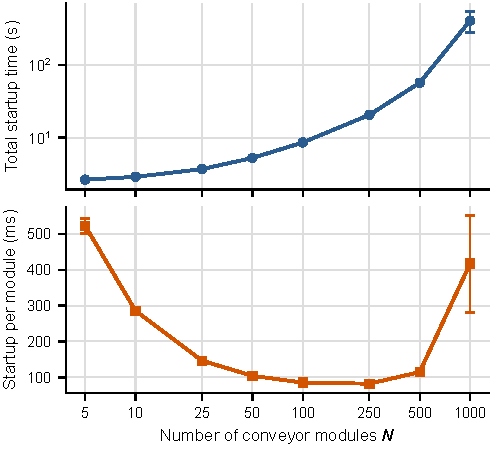
\includegraphics[width=\linewidth]{figures/paper_eval_startup.pdf}
\caption{Total startup time and startup cost per module as a function of the number of conveyor modules.}
\label{fig:eval_startup}
\end{figure}

Rendering performance follows a similar pattern (Fig.~\ref{fig:eval_fps}). Up to 250 modules, the DT runs with ample headroom, with mean frame rates of $460.80$\,FPS at $N=5$, $344.68$\,FPS at $N=50$, and $254.24$\,FPS at $N=250$, and 1\% low values that never fall below $98.9$\,FPS. At $N=500$, the mean of $93.16$\,FPS still exceeds the 60\,FPS target, but the 1\% low drops to $39.0$\,FPS when many workpieces engage belt colliders at the same time and trigger bursts of narrow-phase collision checks. At $N=1000$, the engine saturates, with a mean of $13.96$\,FPS and 1\% low values close to zero. The standard deviation larger than the mean reflects long stalls alternating with short bursts of frames, a sign that the main thread has saturated.

\begin{figure}[t]
\centering
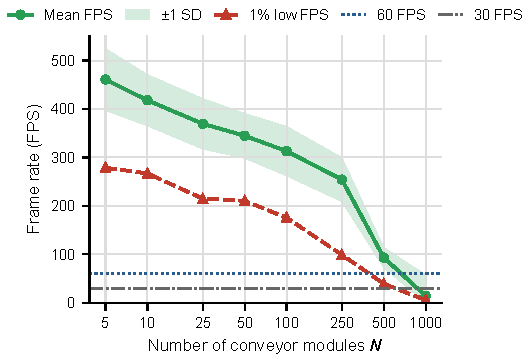
\includegraphics[width=\linewidth]{figures/paper_eval_fps.pdf}
\caption{Mean frame rate, standard deviation, and 1\% low frame rate versus module count, with the 60\,FPS and 30\,FPS thresholds.}
\label{fig:eval_fps}
\end{figure}

The frame cost per module confirms this interpretation. It falls from about $498\,\mu$s at $N=5$ to $66\,\mu$s at $N=50$ and reaches a minimum of $21.7\,\mu$s at $N=250$, as the fixed per-frame work of the engine (loop orchestration, input polling, draw-call setup) is amortized, and then rises sharply to $342.2\,\mu$s at $N=1000$, when pairwise collider checks and contact resolution dominate. Up to $N=250$, all configurations show a short transient during instantiation followed by flat frame rates, with no sign of progressive degradation. Over all 800 runs, frame time correlates with module count ($r = 0.84$), and mean and 1\% low FPS are closely coupled ($r = 0.92$), so frame drops track the overall load rather than appearing as isolated anomalies. The near-perfect correlation between frame time and startup time ($r = 0.99$) is dominated by the $N=1000$ runs and confirms the shared saturation mechanism rather than a linear law over the whole range.

\subsection{Synchronization Analysis}
\label{sec:res_sync}

The two synchronization requirements, low telemetry latency (NFR1) and drift compensation (FR4), follow from the design of the telemetry path. Measuring them directly would require a common time base between the PLC and the workstation, which the ATmega2560 does not provide, so they are estimated here from the timing of each stage, combining the firmware configuration with the frame times measured on the pilot bench. Table~\ref{tab:latency_budget} decomposes the path that a sensor transition follows from the field to the simulation.

\begin{table}[t]
\centering
\caption{Estimated Latency Budget of the Telemetry Path (Plant to Twin).}
\label{tab:latency_budget}
\renewcommand{\arraystretch}{1.2}
\footnotesize
\begin{tabularx}{\columnwidth}{@{}Xrr@{}}
\toprule
\textbf{Stage} & \textbf{Typical (ms)} & \textbf{Worst (ms)} \\
\midrule
Input scan by the sensor task (one tick)          & $\approx 7.5$ & $15$ \\
Queueing, JSON serialization, TCP send (W5500)     & $< 1$         & $\approx 1$ \\
Ethernet transfer of a $<$64\,B message (LAN)      & $< 1$         & $< 1$ \\
Reception thread and concurrent queue              & $< 1$         & $< 1$ \\
Drain at the next frame (pilot bench, Table~\ref{tab:fms_results}) & $2.36$ & $9.94$ \\
\midrule
\textbf{Total (estimated)}                         & $\approx 11$  & $\approx 27$ \\
\bottomrule
\end{tabularx}
\end{table}

The dominant term is the scan period of the firmware, not the network or the runtime: a transition waits on average half a tick, about 7.5\,ms. The second term, the wait until the main thread drains the queue, is bounded by the frame time and is small because the scene runs far above 60\,FPS. The resulting delay, about 11\,ms typically and below 30\,ms in the worst case, is in the order of one 20\,ms physics step. Because the firmware transmits events rather than cyclic snapshots, this budget does not grow with the number of inputs. The opposite direction is not time-critical: a skill request starts a transfer lasting several seconds, so a few milliseconds of HTTP delay are negligible.

The latency budget translates directly into a spatial error: a workpiece moving at speed $v$ advances $\Delta x = v\,\Delta t$ during the delay $\Delta t$, which at the slow belt speeds of the bench is small compared with the size of a module. This error does not accumulate. Every transfer sequence ends with a wait on the sensor of the receiving station, and that wait is released and snapped by the physical sensor. The pose error of a virtual workpiece is therefore reset at every station, and its maximum value is the error accumulated while crossing a single module, regardless of how long the cell operates. 
%=============================================================================
\section{Discussion}
\label{sec:discussion}
%=============================================================================

\subsection{Verification of Research Objectives}
\label{sec:disc_verification}

The evaluation addresses the research question along three axes. Regarding semantic asset integration, the proposed AAS submodel schema united 3D geometry, kinematic bounds, virtual I/O pins, and rule-triggered control sequences, and the same AASX packages drove both stand-alone VC and live synchronization with the physical hardware without modifying the asset manifests. Regarding procedural scene assembly, the runtime built all meshes, colliders, and telemetry bindings in memory at launch, in $2.79$\,s for the pilot bench and $5.22$\,s for a 50-module layout, and the case study showed that a new asset joins a running scene within one discovery cycle, with its control sequences active after a reload of about 3\,s. Regarding synchronization and scalability, the estimated end-to-end delay is in the order of one physics step, drift is bounded to a single module (Section~\ref{sec:res_sync}), and real-time operation is stable up to 250 modules, with 500 modules marking the edge of the comfortable operating range. Regarding the remaining requirements, the same registry and repository served up to 1000 shells without any configuration change, which supports NFR2 for a single client, whereas concurrent clients were not evaluated. Layer decoupling (NFR3) follows from the architecture, since after ingestion the storage services are no longer on the execution path, and Conveyor~G was authored and published entirely through forms, without writing code (NFR4).

\subsection{Limitations and Operational Scope}
\label{sec:disc_limitations}

Several limitations must nonetheless be considered. The first is the main-thread bottleneck. The physics step, the contact callbacks, and the controller scripts all run on Unity's main thread, so performance drops to 14\,FPS at 1000 modules. Facilities exceeding 500 active conveyors would require spatial culling or a migration of rigid-body dynamics and controllers to Unity's Data-Oriented Technology Stack (DOTS) and compute shaders. The second is ingestion at large scale. Because ingestion coroutines share the main thread with the running simulation, startup reaches $416.70$\,s at 1000 modules. Batching requests, cooking colliders on worker threads, and deferring physics until ingestion completes would decouple startup from frame time. The third concerns synchronization. Latency and drift were bounded analytically rather than measured, all performance runs were executed in VC mode, the snapping logic assumes a single workpiece per transfer, and changes to \textit{ControlLogic} take effect only when the scene is reloaded. Moreover, although the PLC remains the final executor of every skill requested by the twin, no arbitration is defined for the case in which virtual and physical states disagree, which must be addressed before the approach is used on equipment with safety implications. The fourth is geometric fidelity, since the fast loading times rely on low-polygon models that omit internal manufacturing details. Finally, \textit{VirtualPins} currently models Boolean signals only, so analog sensors and continuously controlled drives are outside the scope of the present schema.

Beyond these limitations, the framework targets discrete manufacturing, where identifiable workpieces move across handling units and trigger binary sensors. Continuous processes, such as chemical refining or thermal processing, are governed by dynamics that rigid-body contact physics cannot represent, and would require coupling the AAS descriptions to co-simulation solvers through standards such as FMI.

%=============================================================================
\section{Conclusion and Future Work}
\label{sec:conclusion}
%=============================================================================

This paper presented an open, model-driven framework that automatically generates and synchronizes simulation-based DTs from standardized Asset Administration Shells. Each asset is described once, in a self-contained AASX package whose five submodels capture its geometry, kinematic behavior, virtual I/O pins, control logic, and network endpoint. Three decoupled layers, preceded by an optional digitization stage in Blender, turn this description into a running twin: no-code authoring, storage and discovery in Eclipse BaSyx~v2, and procedural assembly in Unity~3D with dual-mode execution and sensor-triggered drift correction. On a modular FMS bench, the twin started in $2.79$\,s and ran at about 490\,FPS, while 800 stress-test runs showed stable real-time behavior up to 250 modules and mean frame rates above 60\,FPS up to 500 modules. Once an asset has been described, it can be added to, moved within, or removed from the twin without rebuilding the simulation scene by hand.

Future work will follow several directions. Migrating physics and kinematics to DOTS and GPU compute shaders would remove the main-thread bottleneck observed beyond 500 modules. Encapsulating Unified Robot Description Format (URDF) kinematic trees in AAS submodels and bridging the runtime to the Robot Operating System~2 (ROS~2) would extend the framework to robotic manipulators. Associating each procedural asset with an autonomous software agent would allow modules to announce their capabilities and negotiate routing in a multi-agent plug-and-produce setting \cite{Rocha2024}. Finally, extending the runtime to virtual and augmented reality headsets would support immersive commissioning and operator training.

All software artifacts, submodel schemas, and simulation packages supporting this work are publicly available at \url{https://github.com/TSGouveia/AAS-DT-Framework}.

\bibliographystyle{bibliography/IEEEtranIES}
\bibliography{bibliography/IEEEabrv,bibliography/paper}

\begin{IEEEbiography}[{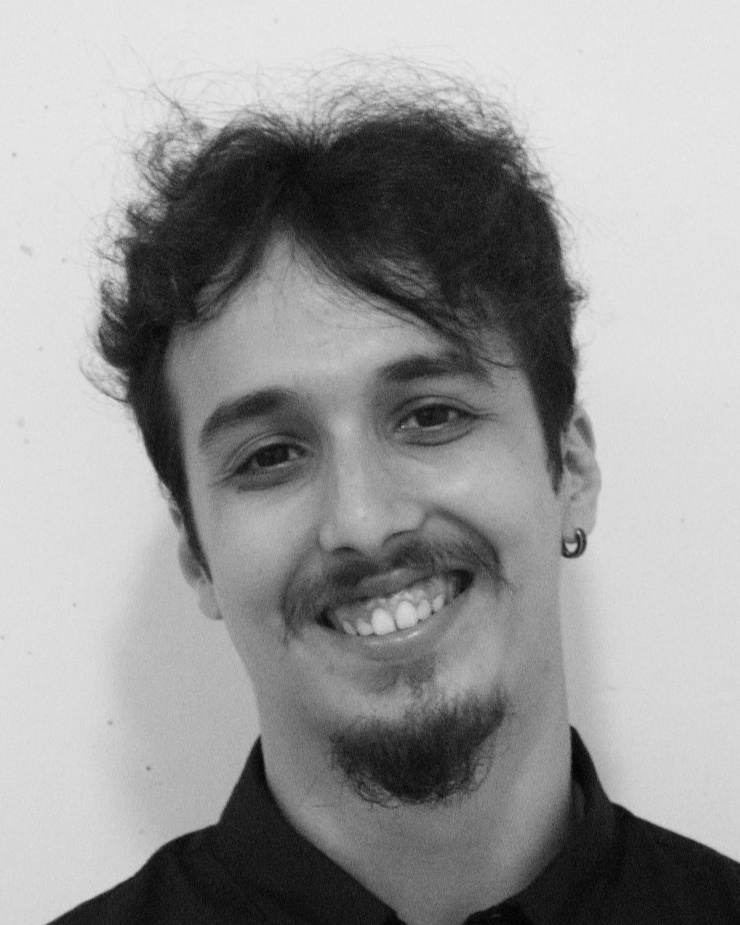
\includegraphics[width=1in,height=1.25in,clip,keepaspectratio]{figures/gouve.jpg}}]{Tiago Gouveia}
% TODO: confirmar dados (grau, ano, interesses)
is currently pursuing the M.Sc. degree in electrical and computer engineering with the NOVA School of Science and Technology (NOVA FCT), NOVA University of Lisbon, Portugal, where he develops his dissertation with the Centre of Technology and Systems (CTS), UNINOVA. His research interests include digital twins, the Asset Administration Shell, virtual commissioning, and the use of game engines for industrial automation and cyber-physical production systems.
\end{IEEEbiography}

\begin{IEEEbiography}[{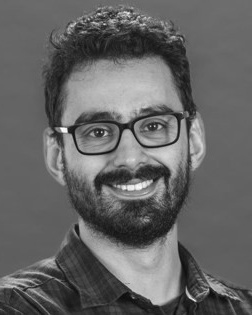
\includegraphics[width=1in,height=1.25in,clip,keepaspectratio]{figures/freit.jpg}}]{Nelson Freitas}
received the M.Sc. degree in electrotechnical and computer engineering from the NOVA School of Science and Technology (NOVA FCT), NOVA University of Lisbon, Portugal, in 2022, where he is currently pursuing the Ph.D. degree in robotics and integrated manufacturing. He is currently an Invited Assistant Professor with the Department of Electrical Engineering, NOVA FCT, and a Fellow Researcher with UNINOVA, Almada, Portugal. He has participated in several research projects at national and European levels, including international projects such as AVANGARD, SmartH4Health, Tech4Green, and COLOSSUS, as well as national projects like ADAM, CESM, and ZDM4MS. His research interests include industrial robotics, industrial data pipelines, digital twins, and smart manufacturing systems. As a result of his research activities, he has published several scientific contributions in peer-reviewed journals and international conference proceedings, co-advised M.Sc. dissertations, and actively contributed to scientific dissemination events, workshops, and peer-review activities.
\end{IEEEbiography}

\begin{IEEEbiography}[{
\includegraphics[width=1in,height=1.25in,clip,keepaspectratio]{figures/rocha.jpg}}]{Andr{\'e} Dion{\'i}sio Rocha}
(Member, IEEE) received the M.Sc. and Ph.D. degrees in electrical and computer engineering from the NOVA University of Lisbon, Portugal, in 2013 and 2018, respectively. He is currently a Professor with the Department of Electrical Engineering, NOVA University of Lisbon, and a Senior Researcher with the Centre of Technology and Systems (CTS), UNINOVA Institute. He has participated in several research projects, most of them at European level (such as H2020 Avangard, H2020 GO0DMAN, H2020 PERFoRM, and H2020 openMOS), involving different programs (FP7, QREN, H2020, and P2020). His research interests include the design and development of cyberphysical production systems and the study of smart manufacturing solutions using distributed control systems, modular production systems, and artificial intelligence-based solutions to deliver more cost-effective and sustainable solutions. As a result of his research activities, he has published several scientific contributions in scientific journals and international conferences. He is highly involved and active in IEEE activities. He is a member of the IEEE-IES Technical Committee on Industrial Cyber-Physical Systems (TCICPS) and the IEEE-IES Technical Committee on Industrial Agents (TC-IA).
\end{IEEEbiography}

\EOD

\end{document}
